

%----------------------------------------------------------------------------------------
%	PACKAGES AND DOCUMENT CONFIGURATIONS
%----------------------------------------------------------------------------------------

\documentclass[12pt,a4paper]{article}

\usepackage[version=3]{mhchem} % Package for chemical equation typesetting
\usepackage{siunitx} % Provides the \SI{}{} and \si{} command for typesetting SI units
\usepackage{graphicx} % Required for the inclusion of images
\usepackage{natbib} % Required to change bibliography style to APA
\usepackage{amsmath} % Required for some math elements 
\usepackage{geometry}
\usepackage{enumerate}
\usepackage{textcomp}
\usepackage{siunitx}
\usepackage{caption}

\renewcommand{\labelenumi}{\alph{enumi}.} % Make numbering in the enumerate environment by letter rather than number (e.g. section 6)
\geometry{left=2cm,right=2cm,top=2.5cm,bottom=2.5cm}

%\usepackage{times} % Uncomment to use the Times New Roman font

%----------------------------------------------------------------------------------------
%	DOCUMENT INFORMATION
%----------------------------------------------------------------------------------------


\begin{document}
\thispagestyle{empty}
\begin{center}

\Large{ \textsc{\newline\rule{14.3cm}{0.05em}\newline\\UM-SJTU Joint Institute\\Physics Laboratory\\(Vp141)\\}}
\rule{14.3cm}{0.05em}
\LARGE{\textsc{\newline\newline\newline\newline\newline\\
Laboratory Report\\}}
\Large{\textsc{  \\ Exercise 5  \\ Damped and Driven Oscillations.\\ Mechanical Resonance\\
} }

\end{center}

\begin{description}
    \item[] 
    \item[] 
    \item[] 
    \item[] 
    \item[] 
    \item[]
    \item[]
    \item[]
    \item[]\qquad \qquad Name: Zhang Yifei \qquad ID:519370910103   \qquad    Group:10
    \item[]\qquad \qquad Date: \today
\end{description}

\newpage
\setcounter{page}{1}

%----------------------------------------------------------------------------------------
%	SECTION 1
%----------------------------------------------------------------------------------------

\section{Introduction}
\subsection{Objectives}
\begin{itemize}
    \item Study damped and driven oscillations in mechanical systems using the Pohl resonator
    \item Observe and quantify the mechanical resonance phenomenon for driven oscillations
\end{itemize}
\subsection{Theoretical Background}
\qquad Forced(driven) oscillation is a kind of motion that a periodically varying external force 
is applied to a damped harmonic oscillator. Assume the driven force is of the form:
\begin{equation}
    F=F_0\cos{\omega t}
    \nonumber
\end{equation}
with the amplitude $F_0$ and angular frequency $\omega$. The resulting steady-state forced 
oscillations will be simple harmonic with the angular frequency equal to that of the driving
force. The amplitude depends on the angular frequency of the driving force, the natural angular 
frequency, and the damping coefficient. A mechanical resonance happens when the amplitude reaches 
maximum, and at that time the phase lag is -$\frac{\pi}{2}$.\par
In this experiment, we'll study  motion of a balance wheel acted by a periodic driving
torque $\tau_{dr}=\tau_0\cos{\omega t}$, a damping torque $\tau_f=-b\frac{d\theta}{dt}$ and a restoring
torque $\tau=-k\theta$, and we can get the equation:
\begin{equation}
    I \frac{d^{2} \theta}{d t^{2}}=-k \theta-b \frac{d \theta}{d t}+\tau_{0} \cos \omega t
\end{equation}
where I is the moment of inertia of the balance wheel, $\tau_0$is the amplitude of the 
driving torque, and $\omega$ is angular frequency of the driving torque, and replace (1) with:
\begin{equation}
    \omega_0^2=\frac{k}{I},\ \ \ \ 2\beta=\frac{b}{I}, \ \ \ \ \mu=\frac{\tau_0}{I},
    \nonumber
\end{equation}
And we can get:
\begin{equation}
    \frac{d^2\theta}{dt^2}+2\beta\frac{d\theta}{dt}+\omega_0^2\theta=\mu\cos{\omega t} \ \ \Rightarrow \ \  \theta(t)=\theta_{tr}(t)+\theta_{st}\cos{(\omega t+\phi)}
    \nonumber
\end{equation}
where the former $\theta_{tr}$ denotes the transient solution, that depends on the initial condition and will
vanish to 0 as t approaches to infinity. $\theta_{st}$ represents the amplitude of steady-state oscillation.
\begin{equation}
    \theta_{st}=\frac{\mu}{\sqrt{(\omega_0^2-\omega^2)^2+4\beta^2\omega^2}}
    \nonumber
\end{equation}
\par Take $\omega=\frac{2\pi}{T}$ and then we can calculate $\beta$ by:
\begin{equation}
    \ln{\frac{\theta_i}{\theta_j}}=\ln{\frac{\theta_0e^{-\beta(iT)}}{\theta_0e^{-\beta(jT)}}}=(j-i)\beta T
\end{equation}
The phase shift $\phi$ can be found as $\tan{\phi}=\frac{2\beta\omega}{\omega^2-\omega_0^2}$ where $-\pi \leq \phi <0$, from this we can get to know that $\phi$ is independent of initial conditions.\par
And finally we can get resonance frequency $\omega=\omega_{res}=\sqrt{\omega_0^2-2\beta^2}$, and correspondingly
$\theta_{res}=\theta_{st}(\omega_{res})=\frac{\mu}{2\beta\sqrt{\omega_0^2-\beta^2}}$.
%----------------------------------------------------------------------------------------
%	SECTION 2
%----------------------------------------------------------------------------------------

\section{Experimental setup}

%----------------------------------------------------------------------------------------
\subsection{Apparatus}
\qquad In this experiment, a BG-2 Pohl resonator is used. The BG-2 Pohl resonator consists of two 
main parts: a vibrometer and a control box. The setups of the vibrometer and the control
 box are shown respectively in figure 4 and 5 in appendix 1.
\par The BG-2 Pohl resonator can measure amplitude, time period, and phase lag.
\par The amplitude of oscillations is measured by counting the notches on the wheel, and 
this measurement is performed by a photoelectric detector with the result displayed on the 
electronic control box. After pressing the button, the timer on the control box 
will start to count the time. The measurement of time 
has an uncertainty of 0.001s and the uncertainty of the amplitude is 1\textdegree.
\par The phase shift can be measured using the glass turntable with an angle scale 
and a strobe light. The strobe is controlled by the photoelectric detector above 
the wheel. When the deep notch passes the equilibrium position, the detector sends a 
signal and the strobe flashes. In a steady state, a line on the angle scale will be 
highlighted by the flash of the strobe and the phase difference can be read from the 
angle scale directly. The phase lag has an uncertainty of 1\textdegree.
The collection of uncertaintes of each device is given in Table 1.
\begin{table}[h]
    \centering
    \begin{tabular}{c|c}
    \textbf{Measurements} & \textbf{Uncertainty} \\ \hline
    Time                  & 0.001s               \\
    Amplitude ($\theta$)            & 1\textdegree                \\
    Phase lag ($\phi$)            & 1\textdegree       
    \end{tabular}
    \caption{Device Uncertainty}
\end{table}


%---------------------------------------------------------------------
%SECTION 4
%---------------------------------------------------------------------
\section{Measurement Procedure}
\subsection{Natural Angular Frequency}
\begin{enumerate}[1.]
    \item After selecting the mode, rotate the balance wheel to the initial angular position
    $\theta_0\approx 90^{\circ}$ and record the period on the panel.
    \item Repeat for four times and calculate the natural angular frequency $\omega_0$.
\end{enumerate}
\subsection{Damping Coefficient}
\begin{enumerate}[1.]
    \item Select damping mode 2, rotate the balance wheel like section 1. Record the period for
ten periods and the amplitdue of each period with the help of "recall".
    \item Calculate the damping coefficient $\beta$ by recalling function(2) in the theoretical backgroud part.
    \begin{equation}
        \ln{\frac{\theta_i}{\theta_j}}=\ln{\frac{\theta_0e^{-\beta(iT)}}{\theta_0e^{-\beta(jT)}}}=(j-i)\beta T \ \ \ \ \Rightarrow \ \ \ \ \beta=\frac{1}{5T}\ln{\frac{\theta_i}{\theta_{i+5}}}
        \nonumber
    \end{equation}
\end{enumerate}
\subsection{$\theta_{st}$ vs. $\omega$ and $\phi$ vs. $\omega$ Characteristics of Forced Oscillations}
\begin{enumerate}[1.]
    \item Keep the damping selection at 2 and set the speed of the motor. Record the amplitdue $\theta_{st}$
    ,the period T and the phase shift $\phi$ after reaching steady-state.
    \item Change the speed of the motor and repeat step 1 about 15 times.
    \item Choose damping selection 1 or 3, repeat the above steps.
    \item Plot the $\theta_{st}(\omega)$ and $\phi(\omega)$ characteristics with $\omega/\omega_{0}$ on the horizontal axis.
\end{enumerate}
%----------------------------------------------------------------------------------------
%	SECTION 5
%----------------------------------------------------------------------------------------

\section{Results}
\subsection{Measurement of Natural Angular Frequency}
\qquad To get natural angular frequency, we measure the time of period. The values are calculated based on table 2.
\begin{table}[h]
    \centering
    
    \begin{tabular}{|c|c|}
    \hline
     & T[s]$\pm$0.001[s]     \\ \hline
    1            & 1.557 \\
    2            & 1.557 \\
    3            & 1.557 \\
    4            & 1.557 \\
    \hline
    \end{tabular}
    \captionsetup[table]{labelsep=space}
    \caption{}
\end{table}
\par That gives the value of the period to be $T=1.557\pm 0.001[s]$ (Detailed calculation for part 4 is put in appendix)
\par And the relative uncertainty is $0.06\%$.
\par Hence the natural frequency can be calculated by $\omega_0=2\pi/T=4.030\pm 0.003[s^{-1}]$ with the 
relative uncertainty of $0.06\%$
\subsection{Damping Coefficient}
\qquad The measurements of damping coefficient is shown in 3.2. The values are calculated
based on Table 3. 
\begin{table}[h]
    \centering
    \begin{tabular}{|c|c|c|c|c|}
    \hline
    \multicolumn{2}{|c|}{Amplitude[\textdegree]$\pm$ 1[\textdegree]}           & \multicolumn{2}{c|}{Amplitude[\textdegree]$\pm$ 1[\textdegree]}    &    $\ln{(\theta_i/\theta_{i+5})}$   \\\hline
              $\ \ \ \theta_0\ \ \ $           & 80 &  $\ \ \ \theta_5 \ \ \  $       & 47 & 0.532 \\\hline
              $\ \ \ \theta_1\ \ \ $         & 72 &   $ \ \ \ \theta_6 \ \ \  $     & 42 & 0.539 \\\hline
              $\ \ \ \theta_2\ \ \  $         & 65 & $\ \ \  \theta_7  \ \ \   $      & 38 & 0.537 \\\hline
              $\ \ \ \theta_3 \ \ \  $        & 58 &  $  \ \ \  \theta_8 \ \ \  $     & 34 & 0.534 \\\hline
              $\ \ \ \theta_4 \ \ \  $         & 51 &  $\ \ \ \theta_9  \ \ \   $     & 30 & 0.531 \\\hline
    \multicolumn{4}{|c|}{The average value of} & 0.535\\\hline
    \end{tabular}
    \captionsetup[table]{labelsep=space}
    \caption{}
\end{table}
\par We need to measure the time of 10 periods and the amplitude of each of them.
The result is shown as follow and the uncertainty of q ($\ln{(\theta_i/\theta_{i+5})}$) 
is 0.006. \par
Since the measurement for 10 periods is $T_{10}=15.595\pm 0.001s$, then T=$1.5595\pm 0.0001s$.
\par Then we can calculated $\beta$ by 
\begin{equation}
    \centering
    \beta=\frac{1}{5T}\ln{\frac{\theta_i}{\theta_{i+5}}}=0.069\pm0.005s^{-1}
    \nonumber
\end{equation}
and the relative uncertainty is $7.3\%$
\subsection{The $\theta_{st}-\omega$ and $\phi-\omega$ Characteristics of Forced Oscillations}
\qquad In this section, we calculate the value of $\omega/\omega_0$ and use this as x-axis.
\par Below are the calculated data used for plotting and the figure. (Raw data, uncertainty and calculations are placed in appendix)
\\\\


\begin{minipage}{\textwidth}

    \begin{minipage}[t]{0.5\textwidth}
    \makeatletter\def\@captype{table}
    \begin{tabular}{|c|c|c|c|}
        \hline
         \multicolumn{2}{|c|}{Damping Selection 2}          &      \multicolumn{2}{c|}{Damping Selection 3}      \\ \hline
         $\omega/\omega_0$    &   $\theta_{st}$$\pm$1 [\textdegree]  & $\omega/\omega_0$      & $\theta_{st}$$\pm$1 [\textdegree]  \\ \hline
        1.057 & 36  & 1.057 & 36  \\ \hline
        1.051 & 40  & 1.045 & 44  \\ \hline
        1.045 & 44  & 1.034 & 56  \\ \hline
        1.039 & 50  & 1.022 & 76  \\ \hline
        1.033 & 57  & 1.011 & 108 \\ \hline
        1.022 & 78  & 1.002 & 130 \\ \hline
        1.011 & 113 & 1.001 & 131 \\ \hline
        1.000 & 140 & 1.000 & 132 \\ \hline
        1.014 & 139 & 0.999 & 132 \\ \hline
        1.001 & 140 & 0.998 & 130 \\ \hline
        0.999 & 140 & 0.995 & 126 \\ \hline
        0.998 & 138 & 0.989 & 112 \\ \hline
        0.996 & 135 & 0.984 & 96  \\ \hline
        0.991 & 123 & 0.979 & 82  \\ \hline
        0.981 & 89  & 0.973 & 71  \\ \hline
        0.973 & 72  & 0.968 & 62  \\ \hline
        0.968 & 63  & 0.963 & 55  \\ \hline
        0.963 & 56  &\multicolumn{2}{c|}{}          \\ \hline
        \end{tabular}
    \caption{$\theta_{st}-\omega$ values}
    \label{sample-table}
    \end{minipage}
    \begin{minipage}[t]{0.5\textwidth}
    \makeatletter\def\@captype{table}
    \begin{tabular}{|c|c|c|c|}
        \hline
        \multicolumn{2}{|c|}{Damping Selection 2}          &      \multicolumn{2}{c|}{Damping Selection 3}      \\ \hline
        $\omega/\omega_0$    &   $\phi$$\pm$1 [\textdegree]  & $\omega/\omega_0$      & $\phi$$\pm$1 [\textdegree]  \\ \hline       
        1.057 & -167 & 1.057 & -164 \\ \hline
        1.051 & -165 & 1.045 & -160 \\ \hline
        1.045 & -164 & 1.034 & -155 \\ \hline
        1.039 & -161 & 1.022 & -145 \\ \hline
        1.033 & -157 & 1.011 & -126 \\ \hline
        1.022 & -147 & 1.002 & -99  \\ \hline
        1.011 & -127 & 1.001 & -95  \\ \hline
        1.000 & -90  & 1.000 & -91  \\ \hline
        1.014 & -97  & 0.999 & -87  \\ \hline
        1.001 & -94  & 0.998 & -83  \\ \hline
        0.999 & -86  & 0.995 & -73  \\ \hline
        0.998 & -82  & 0.989 & -57  \\ \hline
        0.996 & -75  & 0.984 & -47  \\ \hline
        0.991 & -62  & 0.979 & -39  \\ \hline
        0.981 & -40  & 0.973 & -33  \\ \hline
        0.973 & -31  & 0.968 & -28  \\ \hline
        0.968 & -26  & 0.963 & -25  \\ \hline
        0.963 & -23  &       \multicolumn{2}{c|}{}     \\ \hline
        
        \end{tabular}
    \caption{$\phi-\omega$ values}
    \label{sample-table}
    \end{minipage}
    \end{minipage}
    \\\par
Use $\omega/\omega_0$ as x-axis, $\theta_{st}$ and $\phi$ as y-axis respectively,
and we can get the graphs (with error bars) as shown below (Figure 1 and Figure 2). 
\par
From the graph of $\theta_{st}$ vs $(\omega/\omega_0)$ we can see when $(\omega/\omega_0)$ is close to 
1, the $\theta_{st}$ (amplitude of the oscillation) reaches maximum, which means the wheel is at mechanical resonance. Also we can find that the line of damping selection 2 is higher than selection 3. Recall that 
\begin{equation}
    \theta_{st}=\frac{\mu}{\sqrt{(\omega_0^2-\omega^2)^2+4\beta^2\omega^2}}
    \nonumber
\end{equation} we can deduce that $\beta_2<\beta_3$
\par We can see whatever the damping is, when $\phi$ is close to -90 \textdegree, the slope
reaches the maximum, where $\omega/\omega_0$ is close to 1, at this time
the wheel reaches mechanical resonance.

\begin{figure}
    \centering 
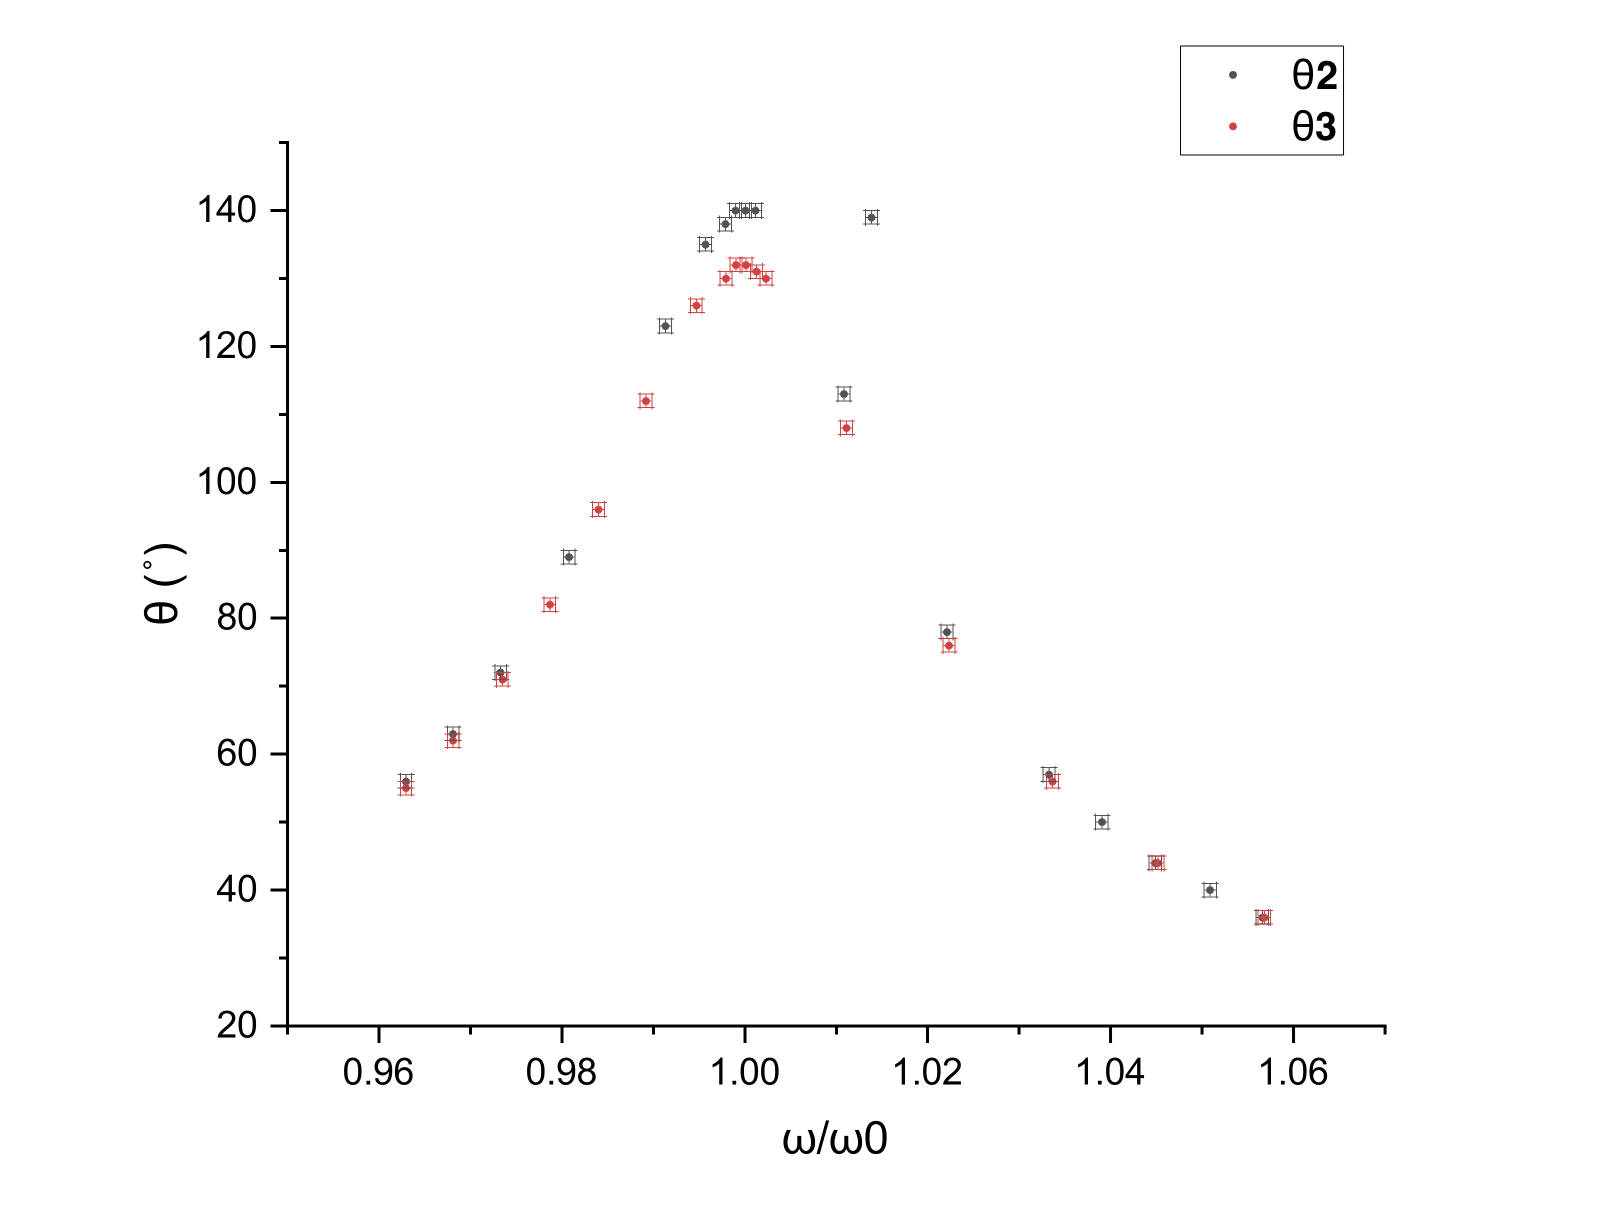
\includegraphics[scale=0.5]{thetanew_new.png}
\caption{graphs of $\theta_{st}$ vs. ($\omega/\omega_0$) }
\end{figure}
\begin{figure}
    \centering
    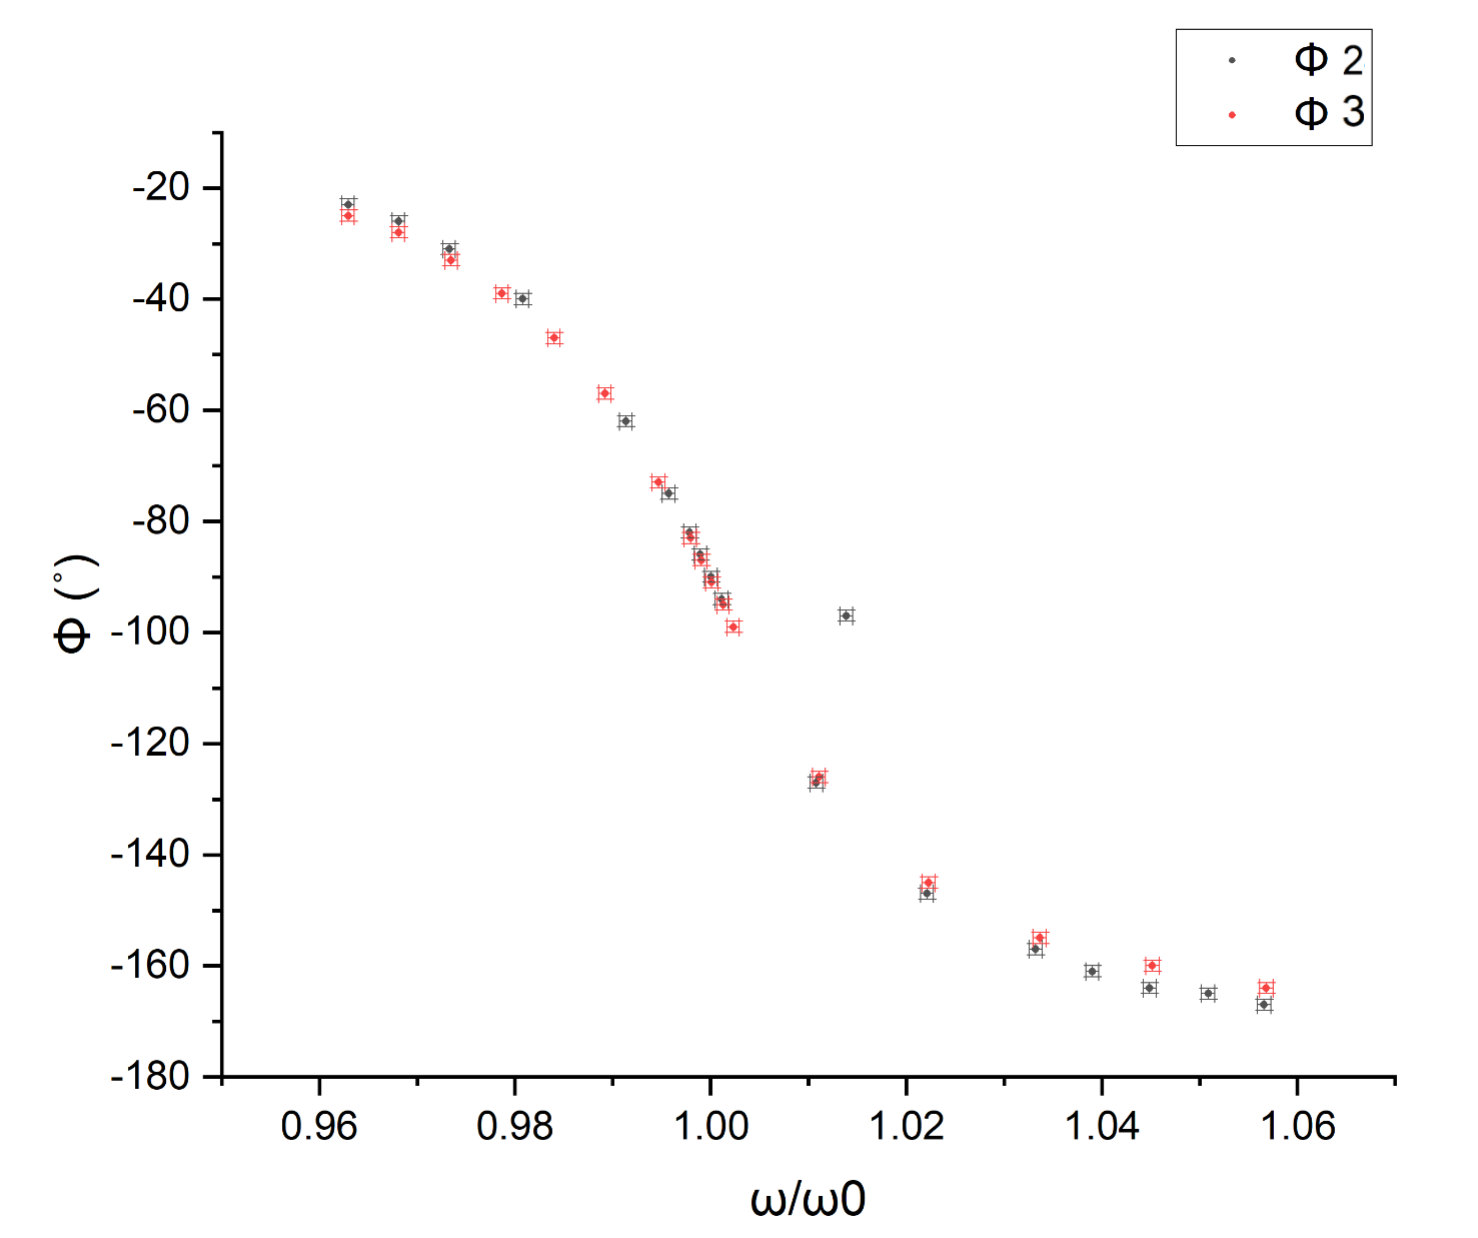
\includegraphics[scale=0.5]{newnewphi.png}
    \caption{graphs of $\phi$ vs. ($\omega/\omega_0$) }
\end{figure}
%----------------------------------------------------------------------------------------
%	SECTION 6
%----------------------------------------------------------------------------------------

\section{Conclusions and Discussion}
%----------------------SUBSECTION1-------------------------------%
\subsection{Summary}
\qquad In this experiment, the natural angular frequency we calculated was:
\begin{equation}
    \omega_0=2\pi/T=4.030\pm 0.003[s^{-1}]
    \nonumber
\end{equation}
with relative uncertainty of $0.06\%$. And the damping coefficient, which is                    
\begin{equation}
    \beta=\frac{1}{5T}\ln{\frac{\theta_i}{\theta_{i+5}}}=0.069\pm0.005s^{-1}
    \nonumber
\end{equation}
with relative uncertainty $7.3\ \%$. And we also plotted the $\theta_{st}$ vs. $\omega/\omega_0$
and $\phi$ vs. $\omega/\omega_0$ graphs to study the characteristics of forced oscillations and get that the value of damping coefficient of selection 2 is smaller than selection 3.
%----------------------SUBSECTION2-------------------------------%
\subsection{Discussions}
\subsubsection{Natural Angular Frequency}
\qquad In this part, we got $0.06\%$ for the relative uncertainty and in the Table 2
we can find that we get four identical values which means this value is very precise.
\par However in this part we neglect the air drag, which actually does have some influence
on the measurement, so the calculated value is slightly smaller than the actual value.
\subsubsection{Damping Coefficient}
\qquad In this part, we got $7.3\%$ for the relative uncertainty, which is non-negligible.
But from calculation we can find that the uncertainty for each element is actually not very large, so 
I think that this uncertainty can be concluded to due to the complex calculation.
\subsubsection{The $\theta_{st}-\omega$ and $\phi-\omega$ Characteristics of Forced Oscillations}
\qquad In this part, we get two figures. For the $\theta_{st}-\omega$ graph (Figure 1) we can see that the value reaches maximum when $\omega/\omega_0$ approaches 1.
And generally the line of damping selection 2 is higher than the line of damping selection 3.
For the $\phi-\omega$ graph (Figure 2) we can find that both lines declines when $\omega/\omega_0$
increases and the slope reaches maximum when $\omega/\omega_0=1$.
\par From figure 4 in appendix which shows the therotical line, we can see that these results generally meets what we expected before the experiment, but quite lower than theoretical line. Recall that:
\begin{equation}
    \theta_{st}=\frac{\mu}{\sqrt{(\omega_0^2-\omega^2)^2+4\beta^2\omega^2}}
    \nonumber
\end{equation}
and we can deduce that $\beta$, with $7.3\%$ relative uncertainty, may be the main cause of this phenomenon. ($\beta$ is larger than theoretical value)
\par It's worth discussing that in both graphs, there is a outlier, which gives by the data that is close to 
resonance. And I think that is because near resonance, the change is not so obvious and I change
too little that the machine can't show the difference at its precision.
\par In this lab experiment, I think there are two parts that create much uncertainty. First is the above part when I change
a little, I can't get precise changes. And the second is the measurement of $\phi$, which will show two values on the machine
and is hard for us to read. So my suggestion is to add precision and use device to read the value of $\phi$.

%----------------------------------------------------------------------------------------
%	SECTION 7
%----------------------------------------------------------------------------------------
\section{Reference}

Qin Tian, Wang Yin, Tianyi Li, Mateusz Krzyzosiak, Physics Laboratory VP141 Exercise 5 Damped and Driven Oscillations.
Mechanical Resonance
%----------------------------------------------------------------------------------------
%	DATASHEET
%----------------------------------------------------------------------------------------

\section*{Appendix \uppercase\expandafter{\romannumeral 1}}
\subsection*{Some Figures}
\begin{figure}[h]
    \centering
    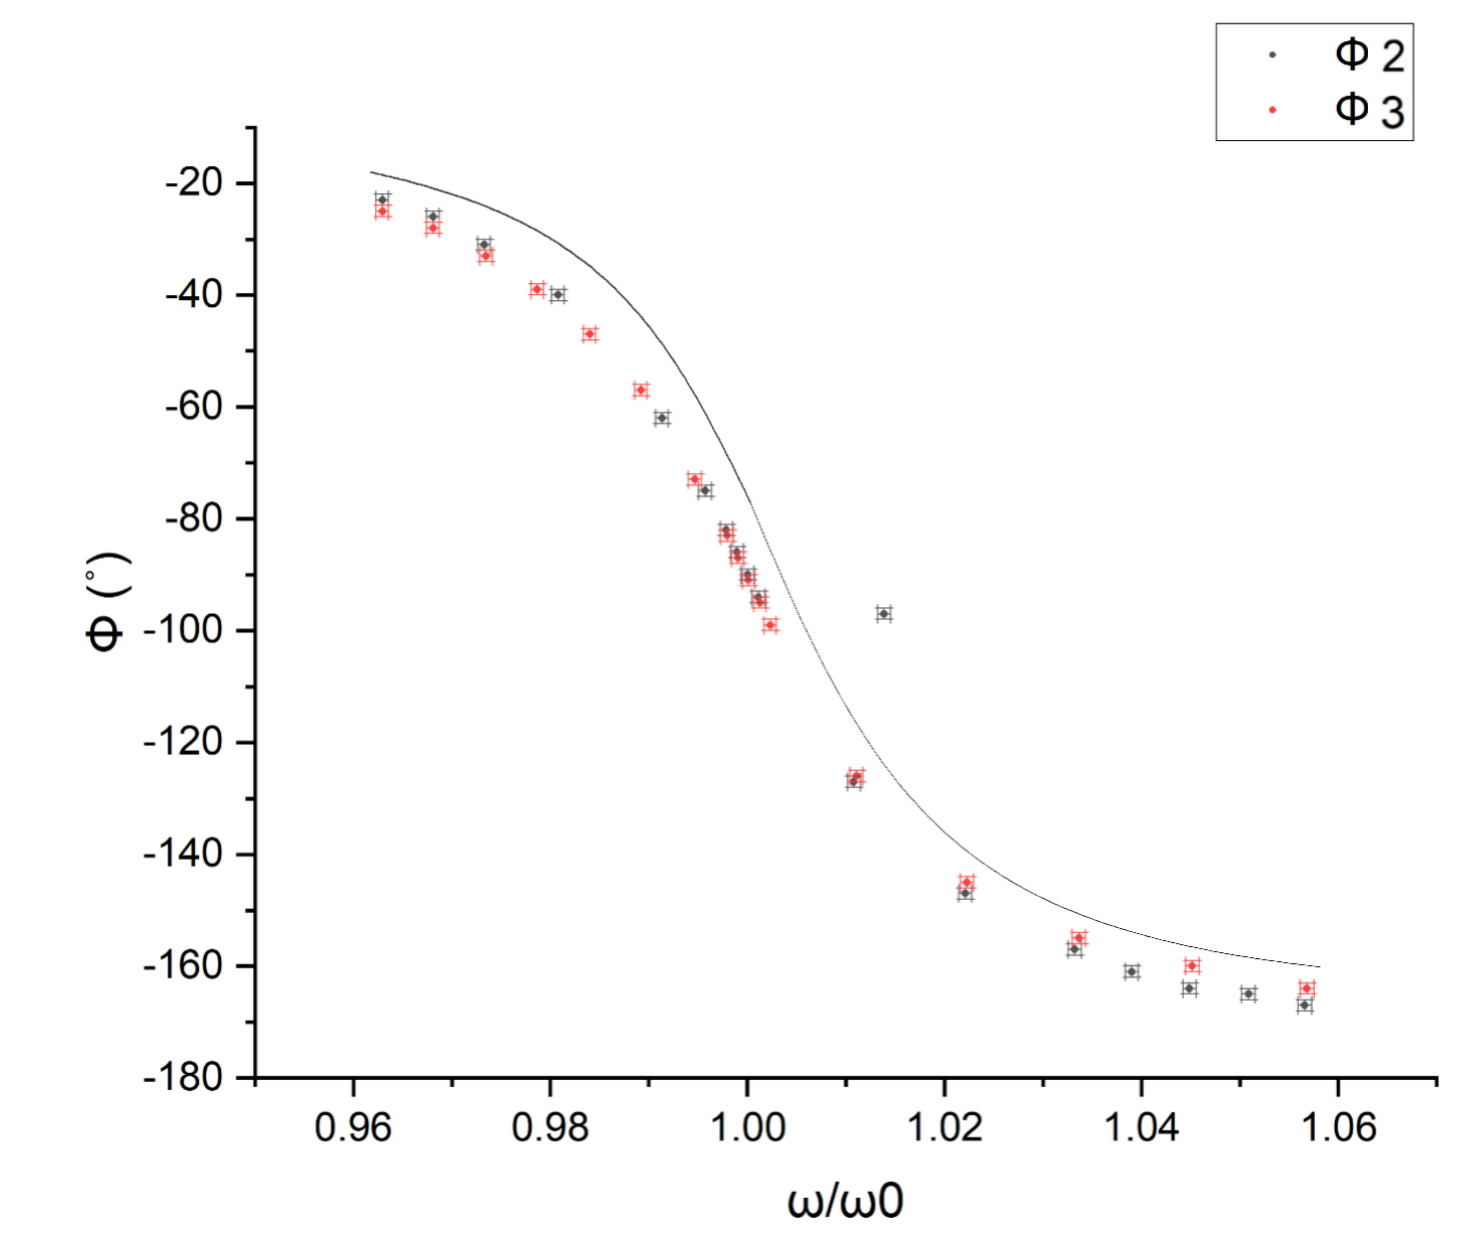
\includegraphics[scale=0.4]{newnewthero.png}
    \caption{theoretical graph}
\end{figure}
\begin{figure}[h]
    \centering
    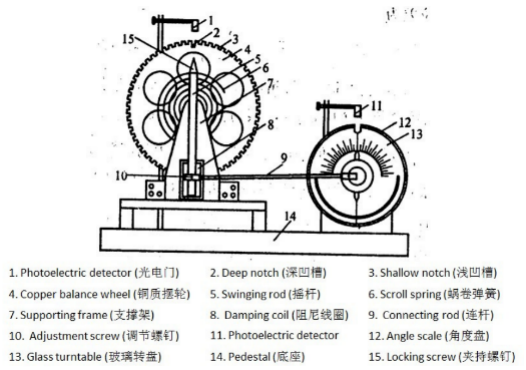
\includegraphics[scale=0.5]{vibrometer.png}
    \caption{vibrometer}
\end{figure}

\begin{figure}[h]
    \centering
    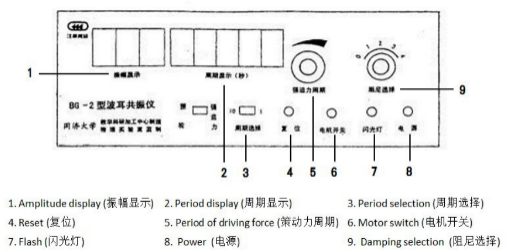
\includegraphics[scale=0.5]{control.png}
    \caption{control box}
\end{figure}

\section*{Appendix \uppercase\expandafter{\romannumeral 2}}
\subsection*{Data and uncertainty analysis}

\begin{table}[h]
    \centering
    \begin{tabular}{|c|c|c|c|c|c|c|}
    \hline
     &$T_{10}$&$T$&$\omega/\omega_0$&uncertainty for $\omega/\omega_0$&$\theta_{st}$$\pm$1 [\textdegree]&$\phi$$\pm$1 [\textdegree]\\ \hline
    1  & 14.736 & 1.4736 & 1.057 & 0.00068 & 167 & -36  \\ \hline
    2  & 14.816 & 1.4816 & 1.051 & 0.00068 & 165 & -40  \\ \hline
    3  & 14.901 & 1.4901 & 1.045 & 0.00067 & 164 & -44  \\ \hline
    4  & 14.985 & 1.4985 & 1.039 & 0.00067 & 161 & -50  \\ \hline
    5  & 15.069 & 1.5069 & 1.033 & 0.00067 & 157 & -57  \\ \hline
    6  & 15.233 & 1.5233 & 1.022 & 0.00066 & 147 & -78  \\ \hline
    7  & 15.403 & 1.5403 & 1.011 & 0.00065 & 127 & -113 \\ \hline
    8  & 15.569 & 1.5569 & 1.000 & 0.00065 & 90  & -140 \\ \hline
    9  & 15.357 & 1.5357 & 1.014 & 0.00065 & 97  & -139 \\ \hline
    10 & 15.552 & 1.5552 & 1.001 & 0.00065 & 94  & -140 \\ \hline
    11 & 15.586 & 1.5586 & 0.999 & 0.00064 & 86  & -140 \\ \hline
    12 & 15.603 & 1.5603 & 0.998 & 0.00064 & 82  & -138 \\ \hline
    13 & 15.637 & 1.5637 & 0.996 & 0.00064 & 75  & -135 \\ \hline
    14 & 15.706 & 1.5706 & 0.991 & 0.00064 & 62  & -123 \\ \hline
    15 & 15.875 & 1.5875 & 0.981 & 0.00063 & 40  & -89  \\ \hline
    16 & 15.997 & 1.5997 & 0.973 & 0.00063 & 31  & -72  \\ \hline
    17 & 16.083 & 1.6083 & 0.968 & 0.00062 & 26  & -63  \\ \hline
    18 & 16.169 & 1.6169 & 0.963 & 0.00062 & 23  & -56  \\ \hline
    \end{tabular}
    \caption{calculated data for damping selection 2}
    \end{table}
%----------------------------------------------------------------------------------------
\begin{table}[h]
    \centering
    \begin{tabular}{|c|c|c|c|c|c|c|}
    \hline
    &$T_{10}$&$T$&$\omega/\omega_0$&uncertainty for $\omega/\omega_0$&$\theta_{st}$$\pm$1 [\textdegree]&$\phi$$\pm$1 [\textdegree]\\ \hline
    1  & 14.733 & 1.4733 & 1.057 & 0.00068 & 164 & -36  \\ \hline
    2  & 14.897 & 1.4897 & 1.045 & 0.00067 & 160 & -44  \\ \hline
    3  & 15.063 & 1.5063 & 1.034 & 0.00067 & 155 & -56  \\ \hline
    4  & 15.23  & 1.523  & 1.022 & 0.00066 & 145 & -76  \\ \hline
    5  & 15.399 & 1.5399 & 1.011 & 0.00065 & 126 & -108 \\ \hline
    6  & 15.534 & 1.5534 & 1.002 & 0.00065 & 99  & -130 \\ \hline
    7  & 15.55  & 1.555  & 1.001 & 0.00065 & 95  & -131 \\ \hline
    8  & 15.568 & 1.5568 & 1.000 & 0.00065 & 91  & -132 \\ \hline
    9  & 15.585 & 1.5585 & 0.999 & 0.00064 & 87  & -132 \\ \hline
    10 & 15.602 & 1.5602 & 0.998 & 0.00064 & 83  & -130 \\ \hline
    11 & 15.653 & 1.5653 & 0.995 & 0.00064 & 73  & -126 \\ \hline
    12 & 15.74  & 1.574  & 0.989 & 0.00064 & 57  & -112 \\ \hline
    13 & 15.823 & 1.5823 & 0.984 & 0.00064 & 47  & -96  \\ \hline
    14 & 15.909 & 1.5909 & 0.979 & 0.00063 & 39  & -82  \\ \hline
    15 & 15.994 & 1.5994 & 0.973 & 0.00063 & 33  & -71  \\ \hline
    16 & 16.083 & 1.6083 & 0.968 & 0.00062 & 28  & -62  \\ \hline
    17 & 16.169 & 1.6169 & 0.963 & 0.00062 & 25  & -55  \\ \hline
    \end{tabular}
    \caption{calculated data for damping selection 3}
    \end{table}

\begin{figure}[t]
    \centering
    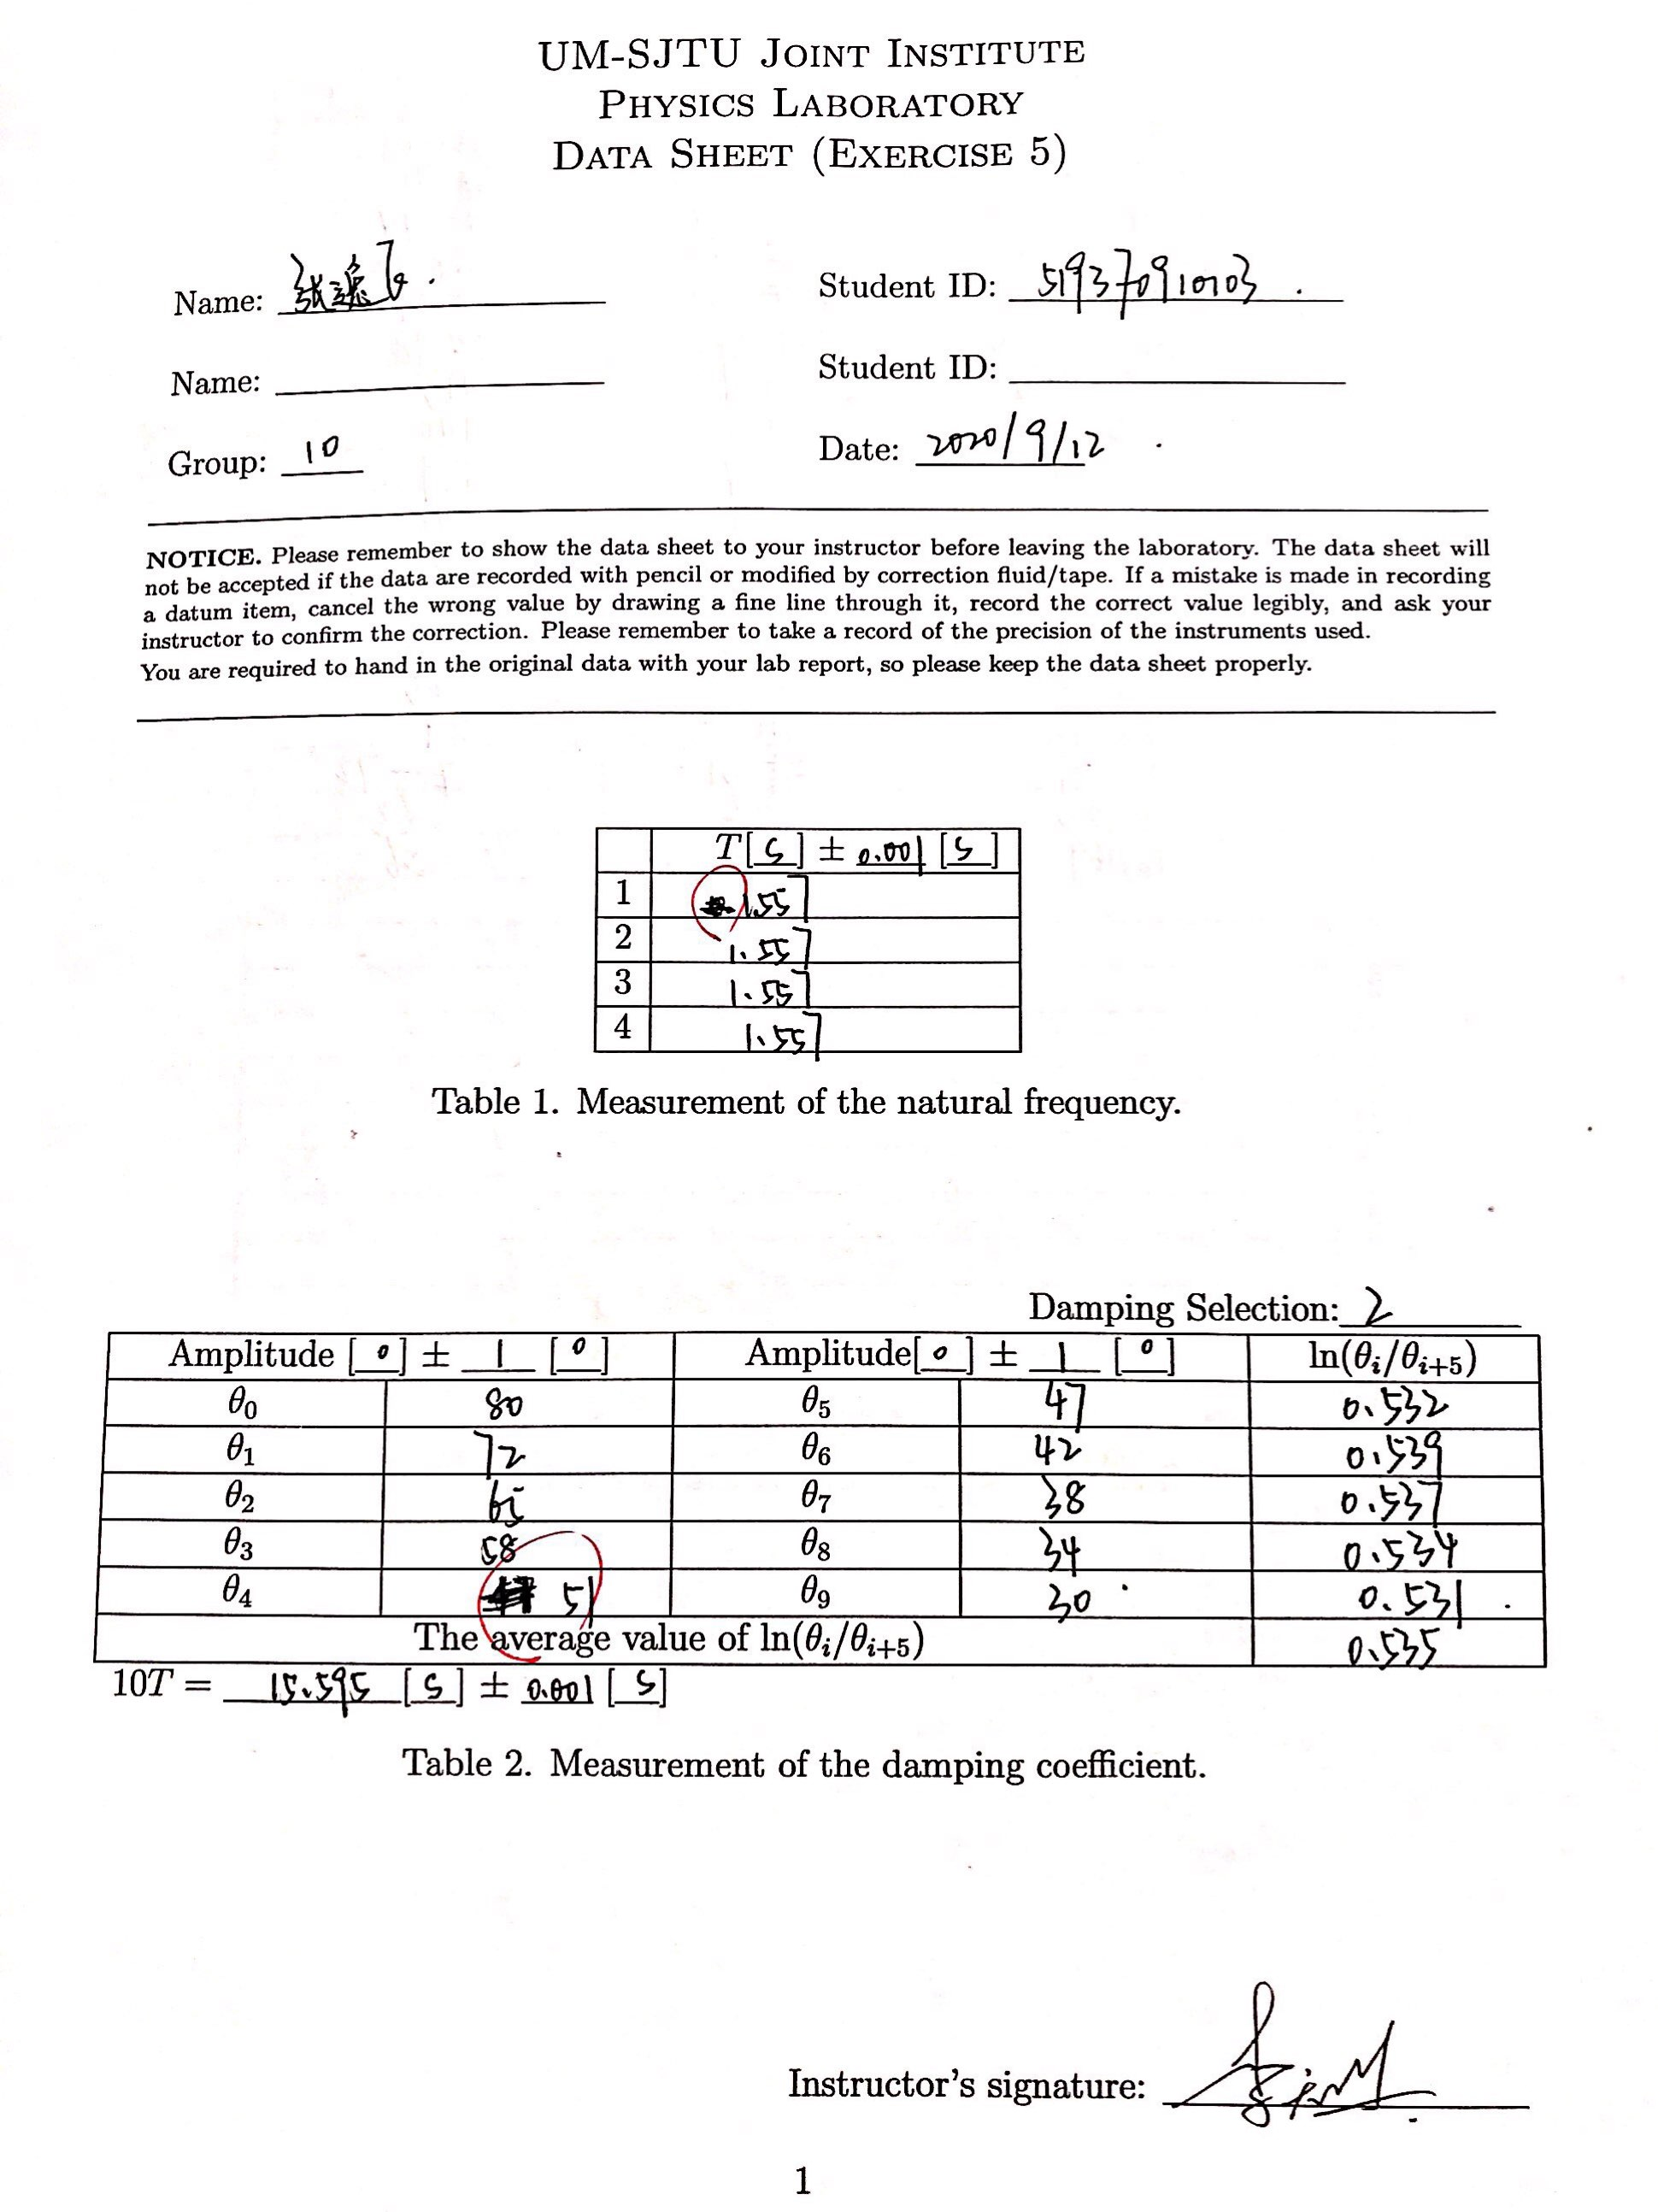
\includegraphics[scale=0.2]{raw1.jpg}
\end{figure}
\begin{figure}[t]
    \centering
    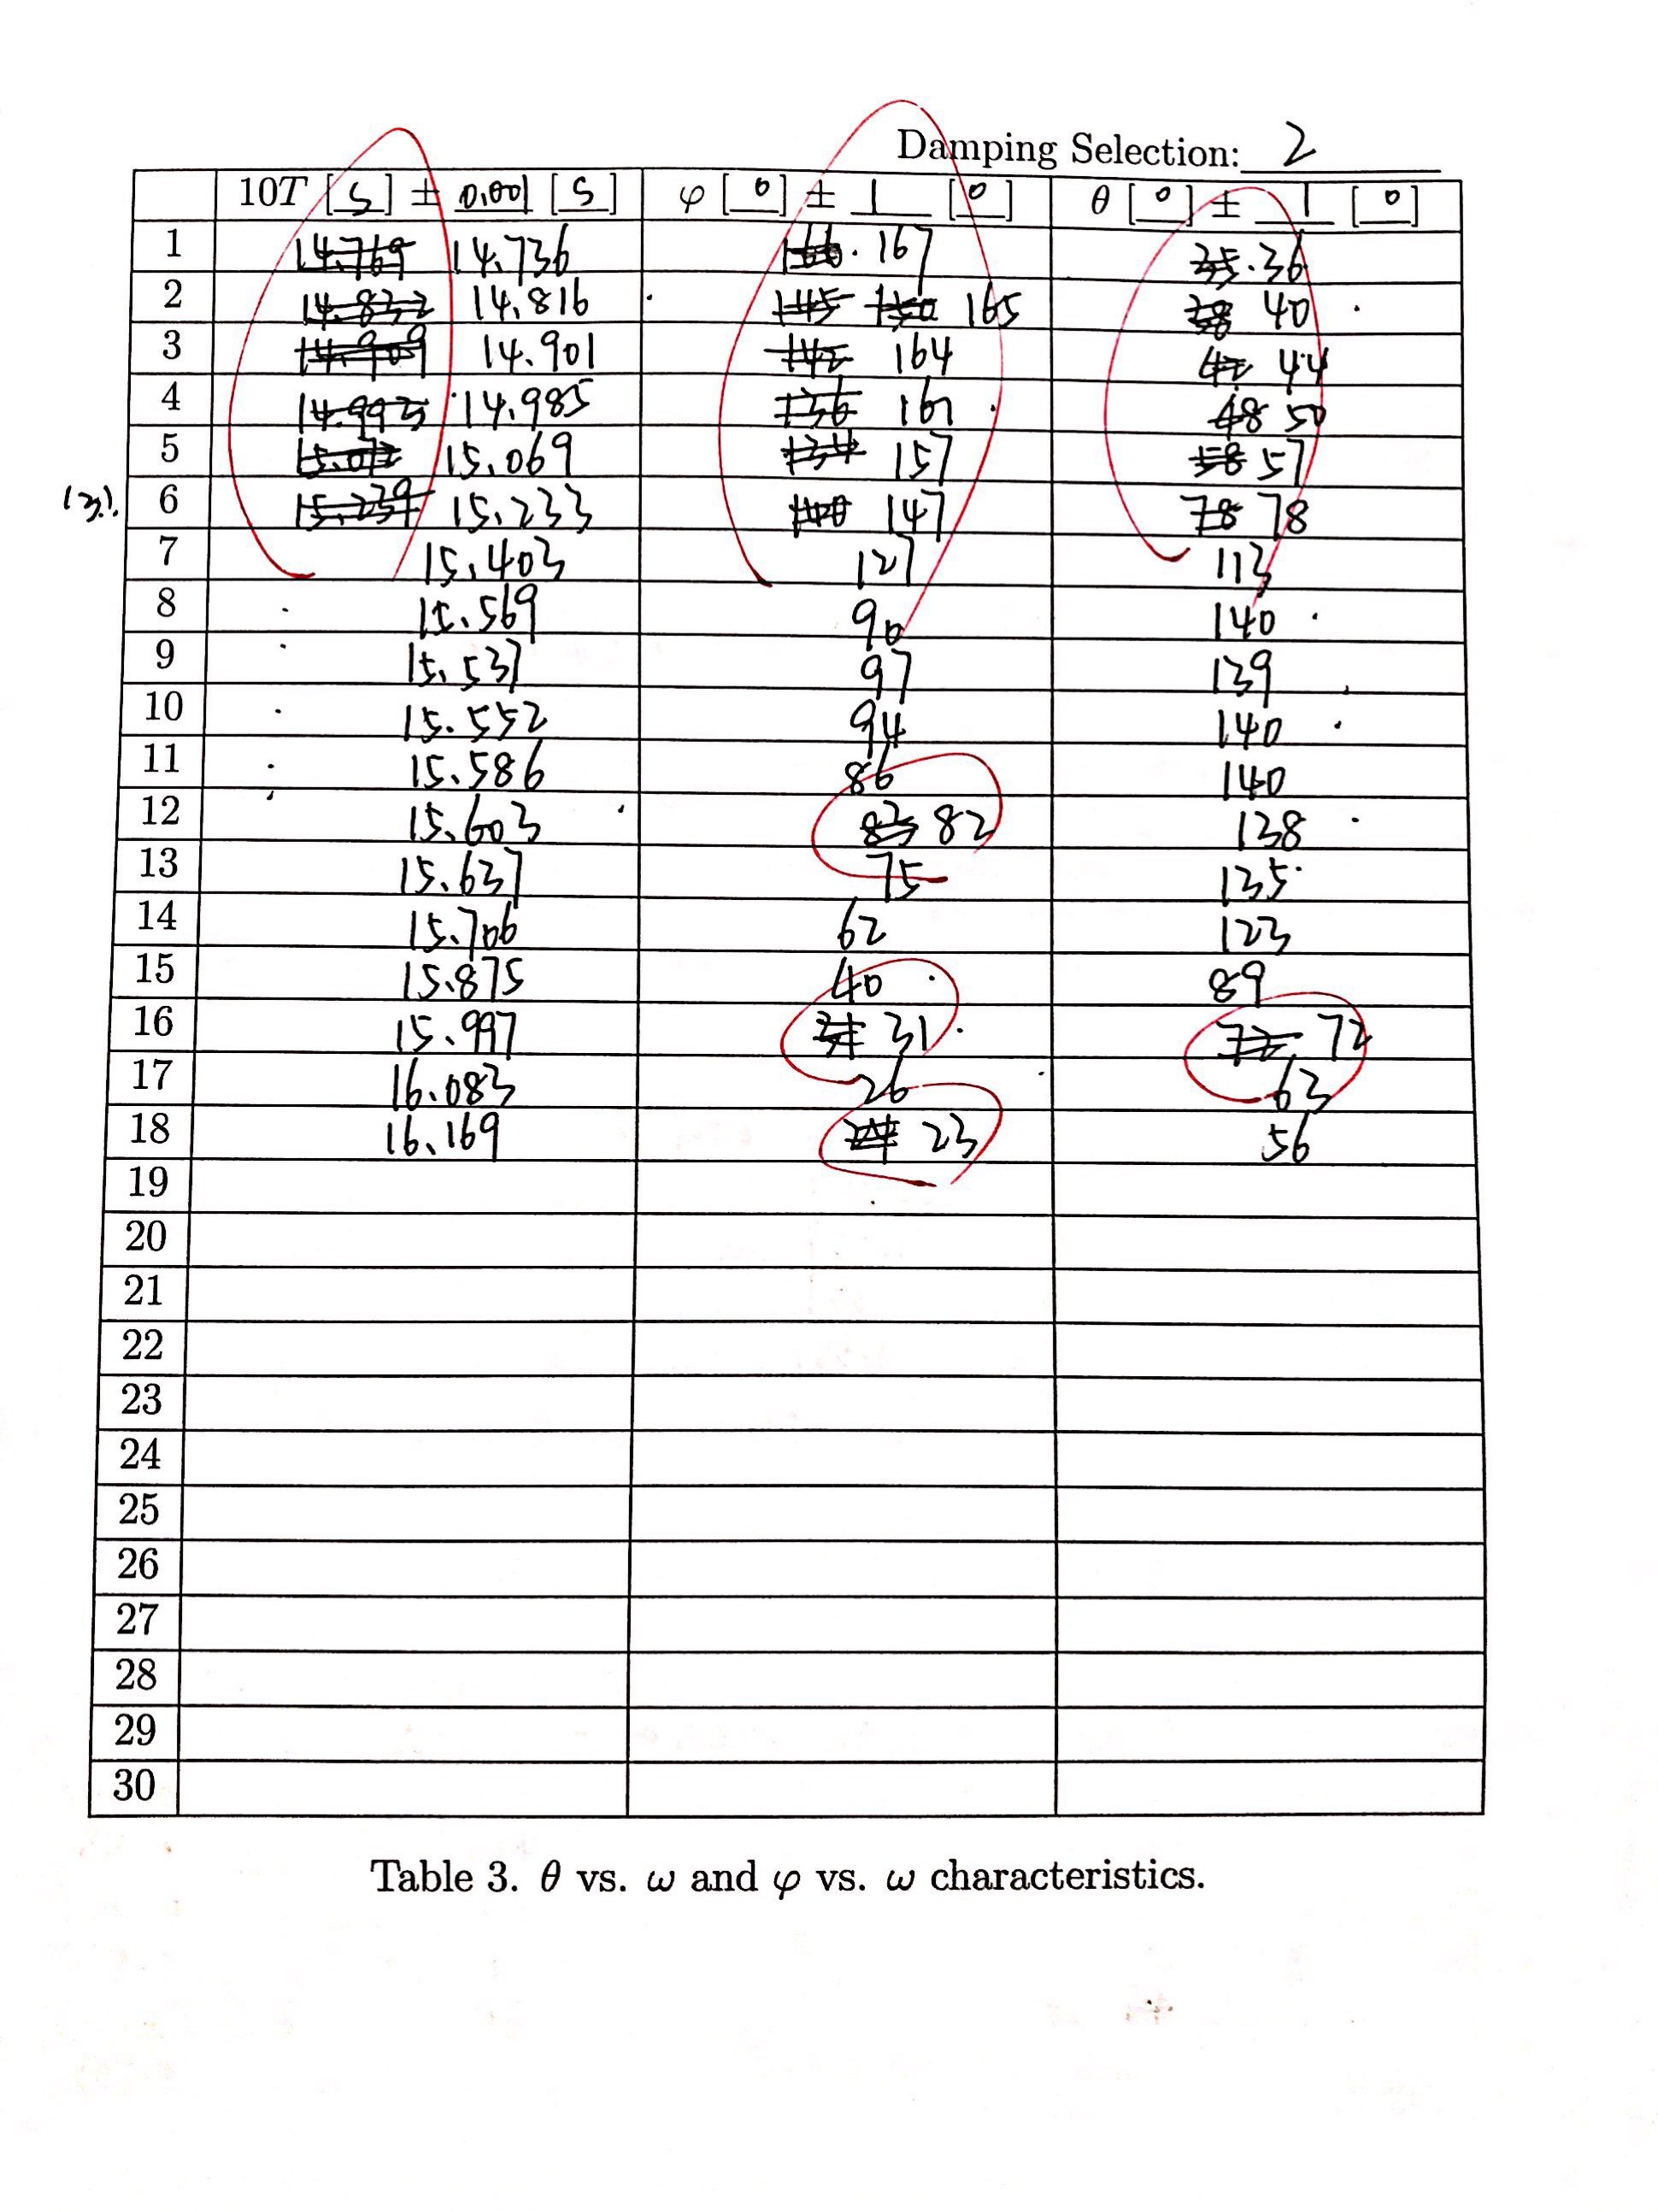
\includegraphics[scale=0.25]{raw2.jpg}
\end{figure}
\begin{figure}[t]
    \centering
    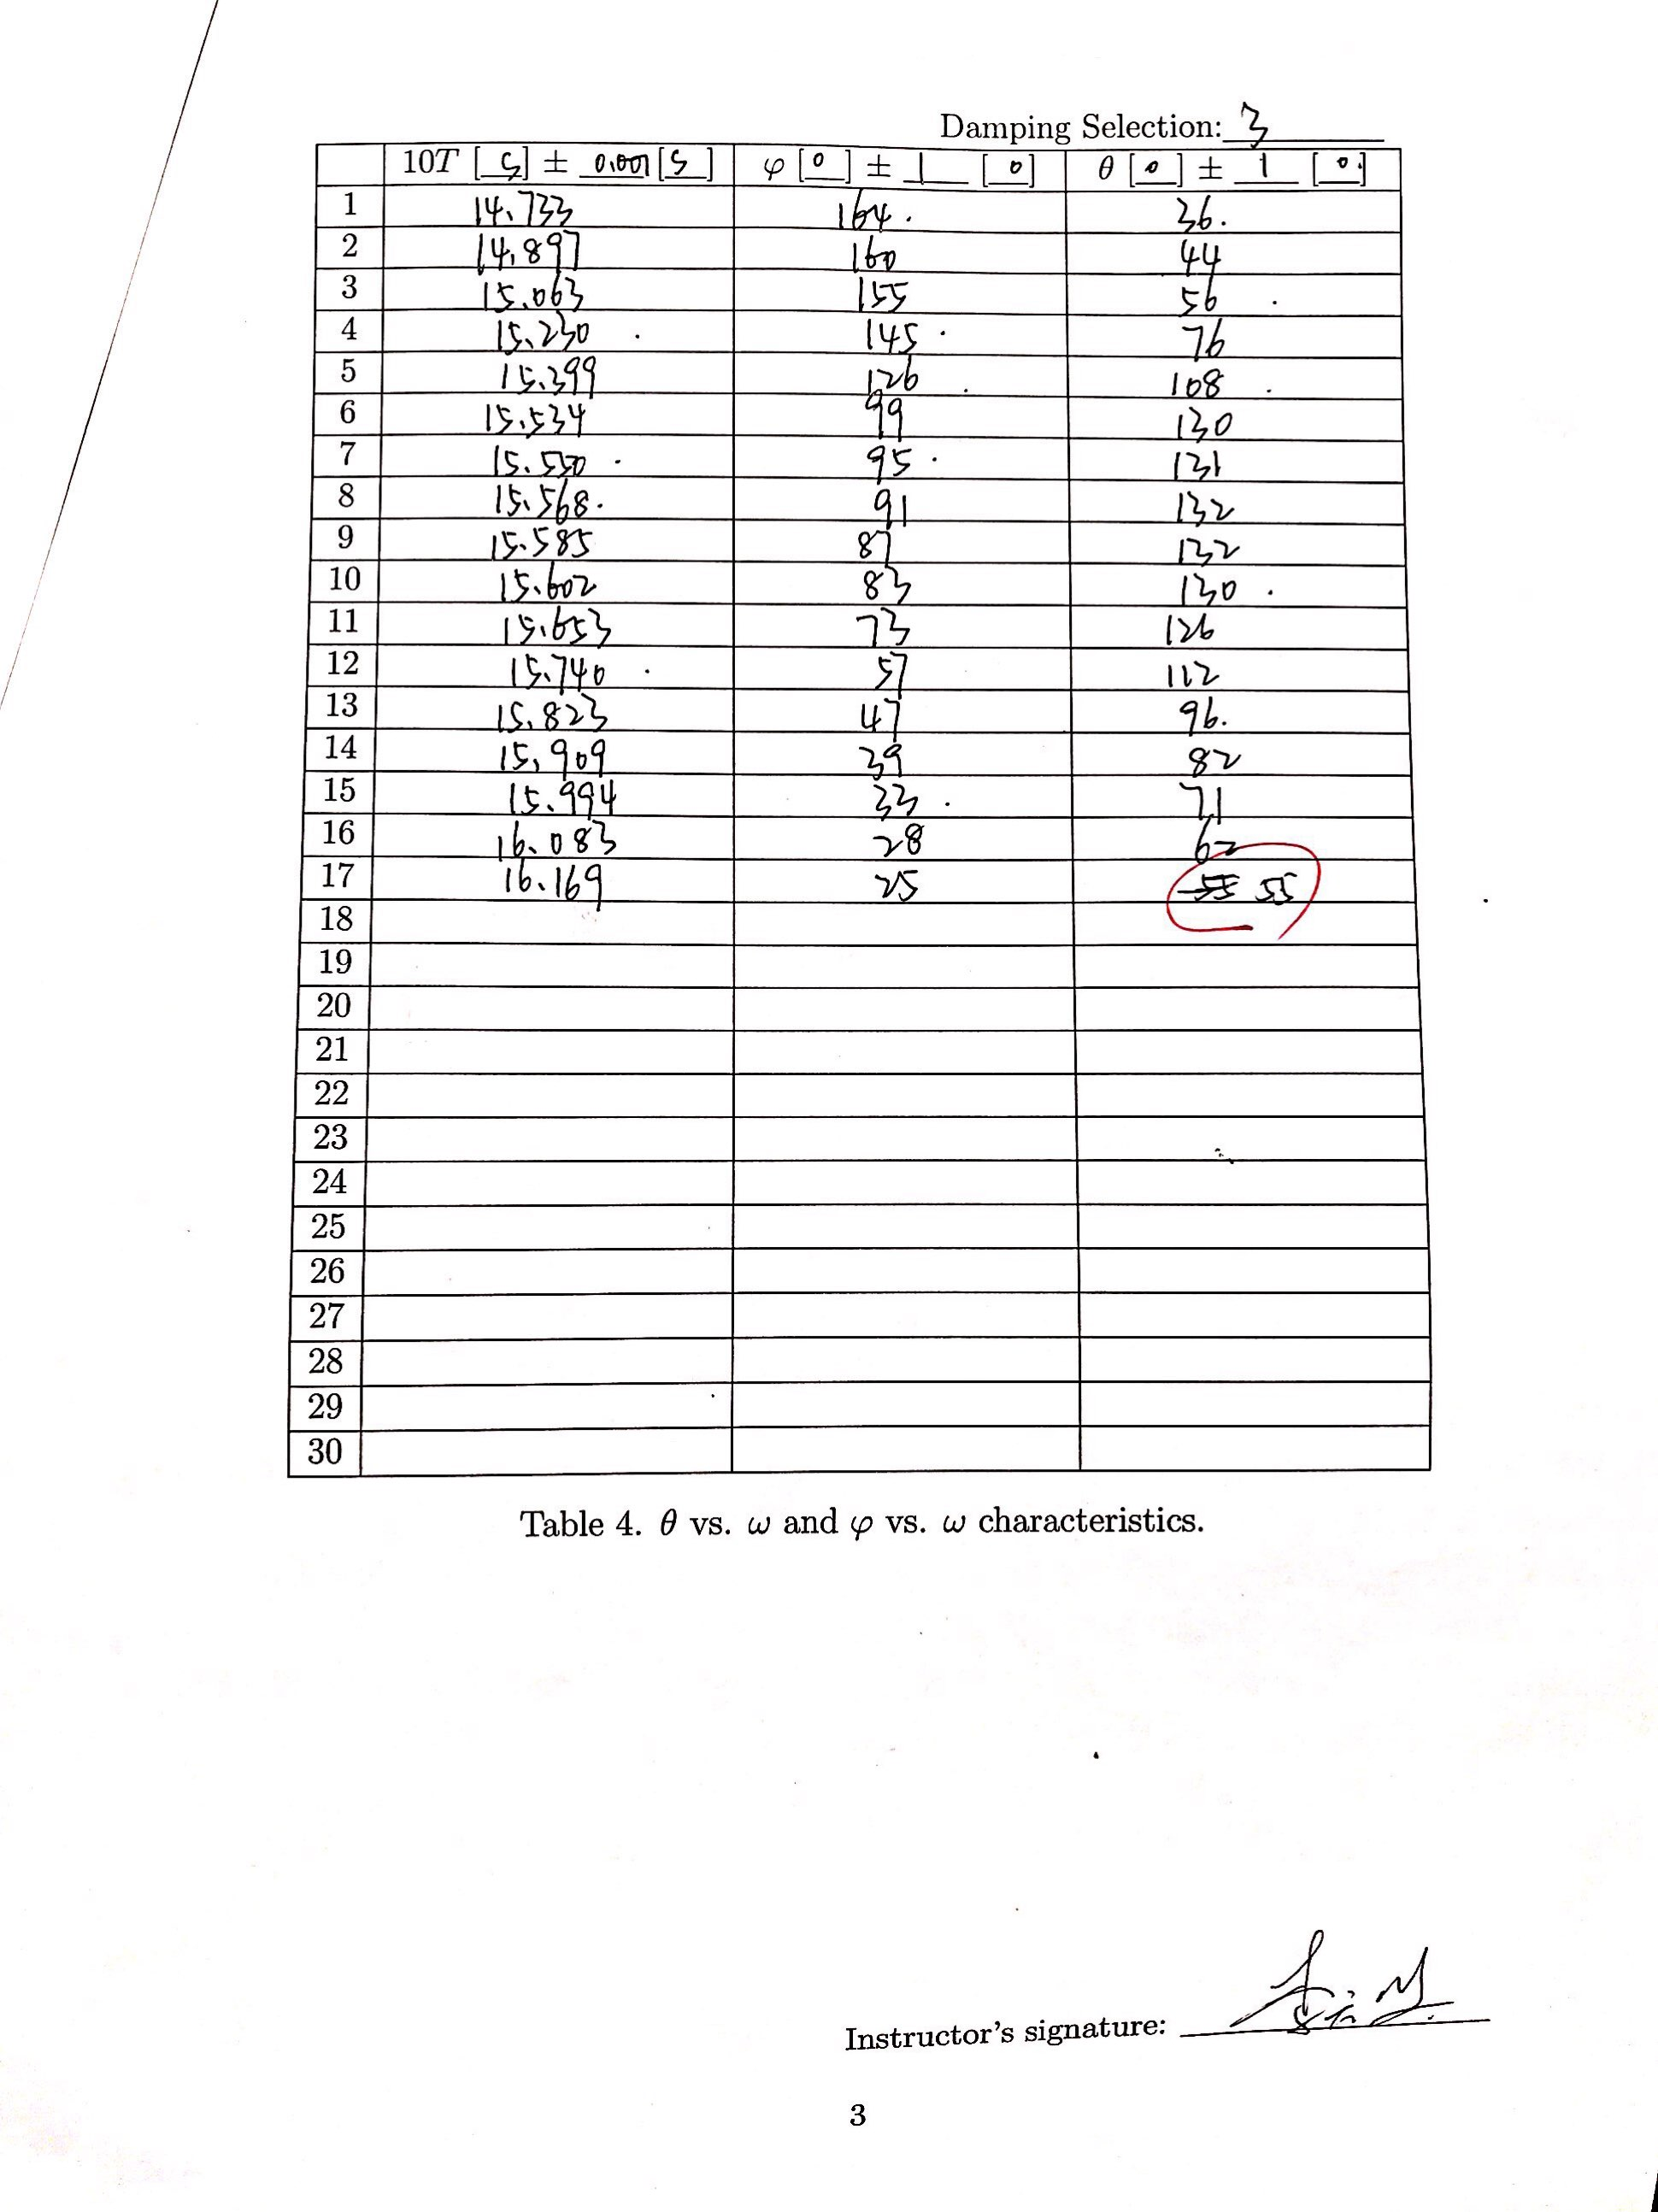
\includegraphics[scale=0.25]{raw3.jpg}
\end{figure}
\begin{figure}[t]
    \centering
    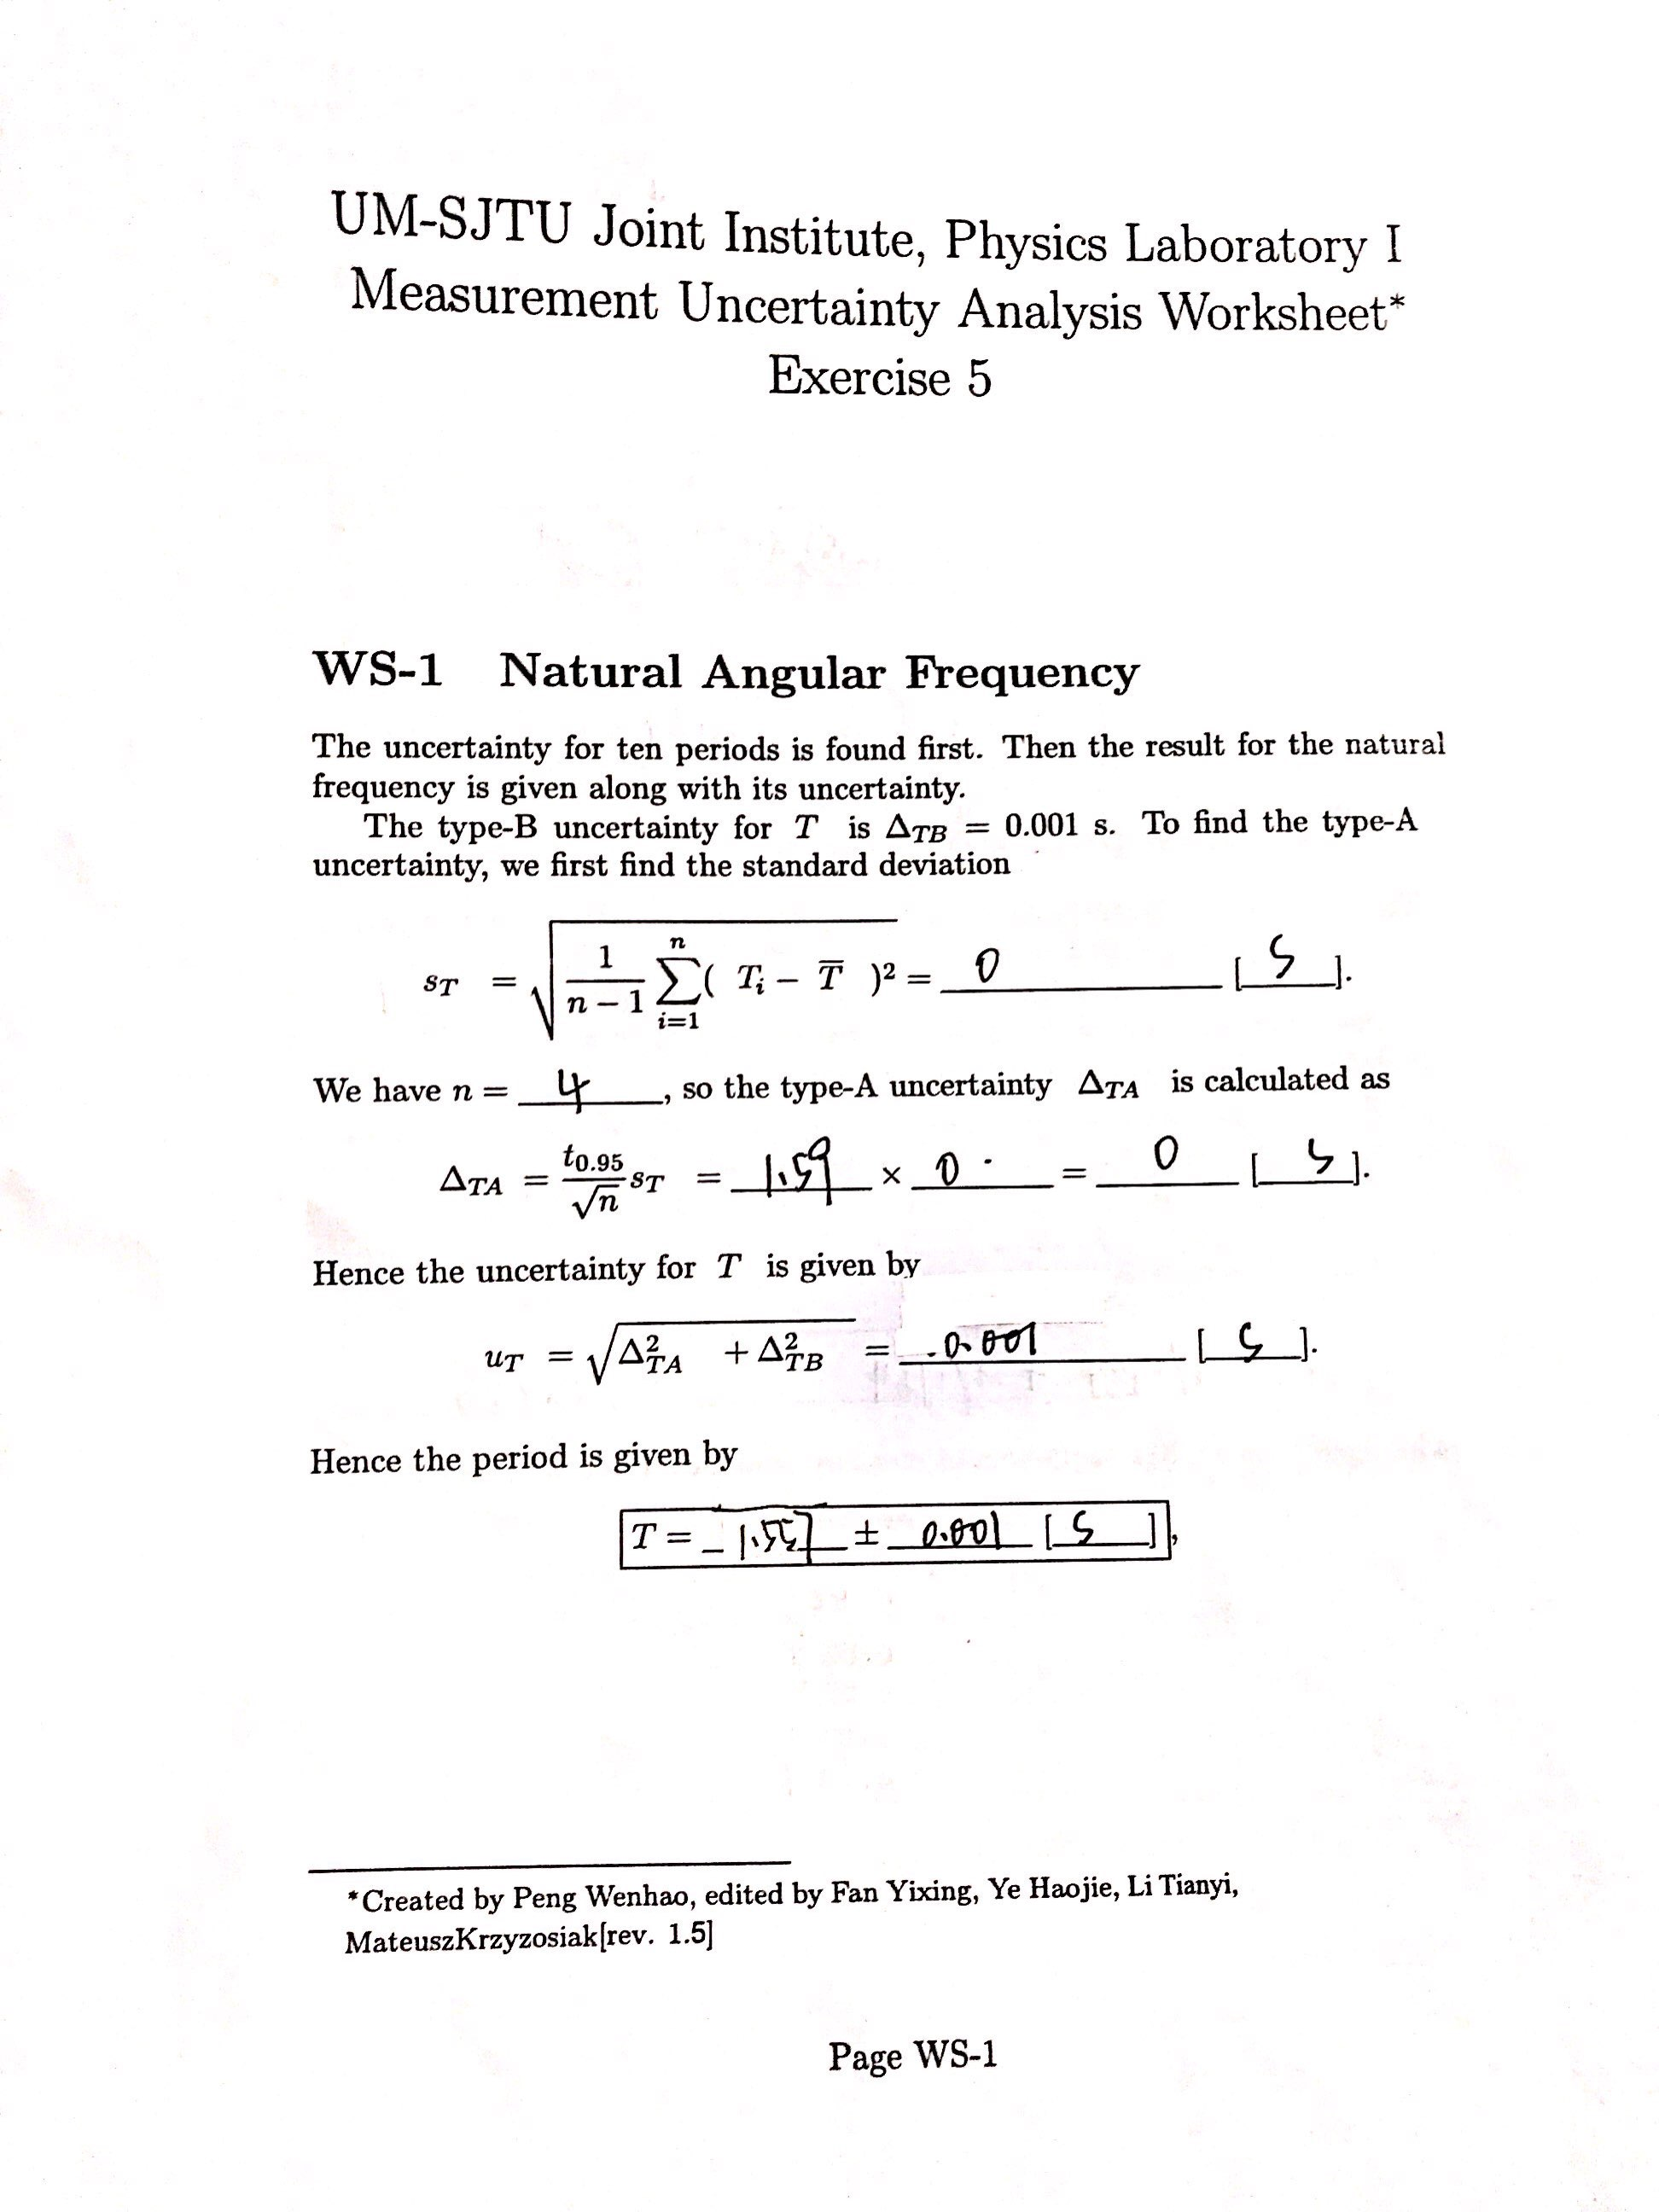
\includegraphics[scale=0.25]{newuncer1.jpeg}
\end{figure}
\begin{figure}[t]
    \centering
    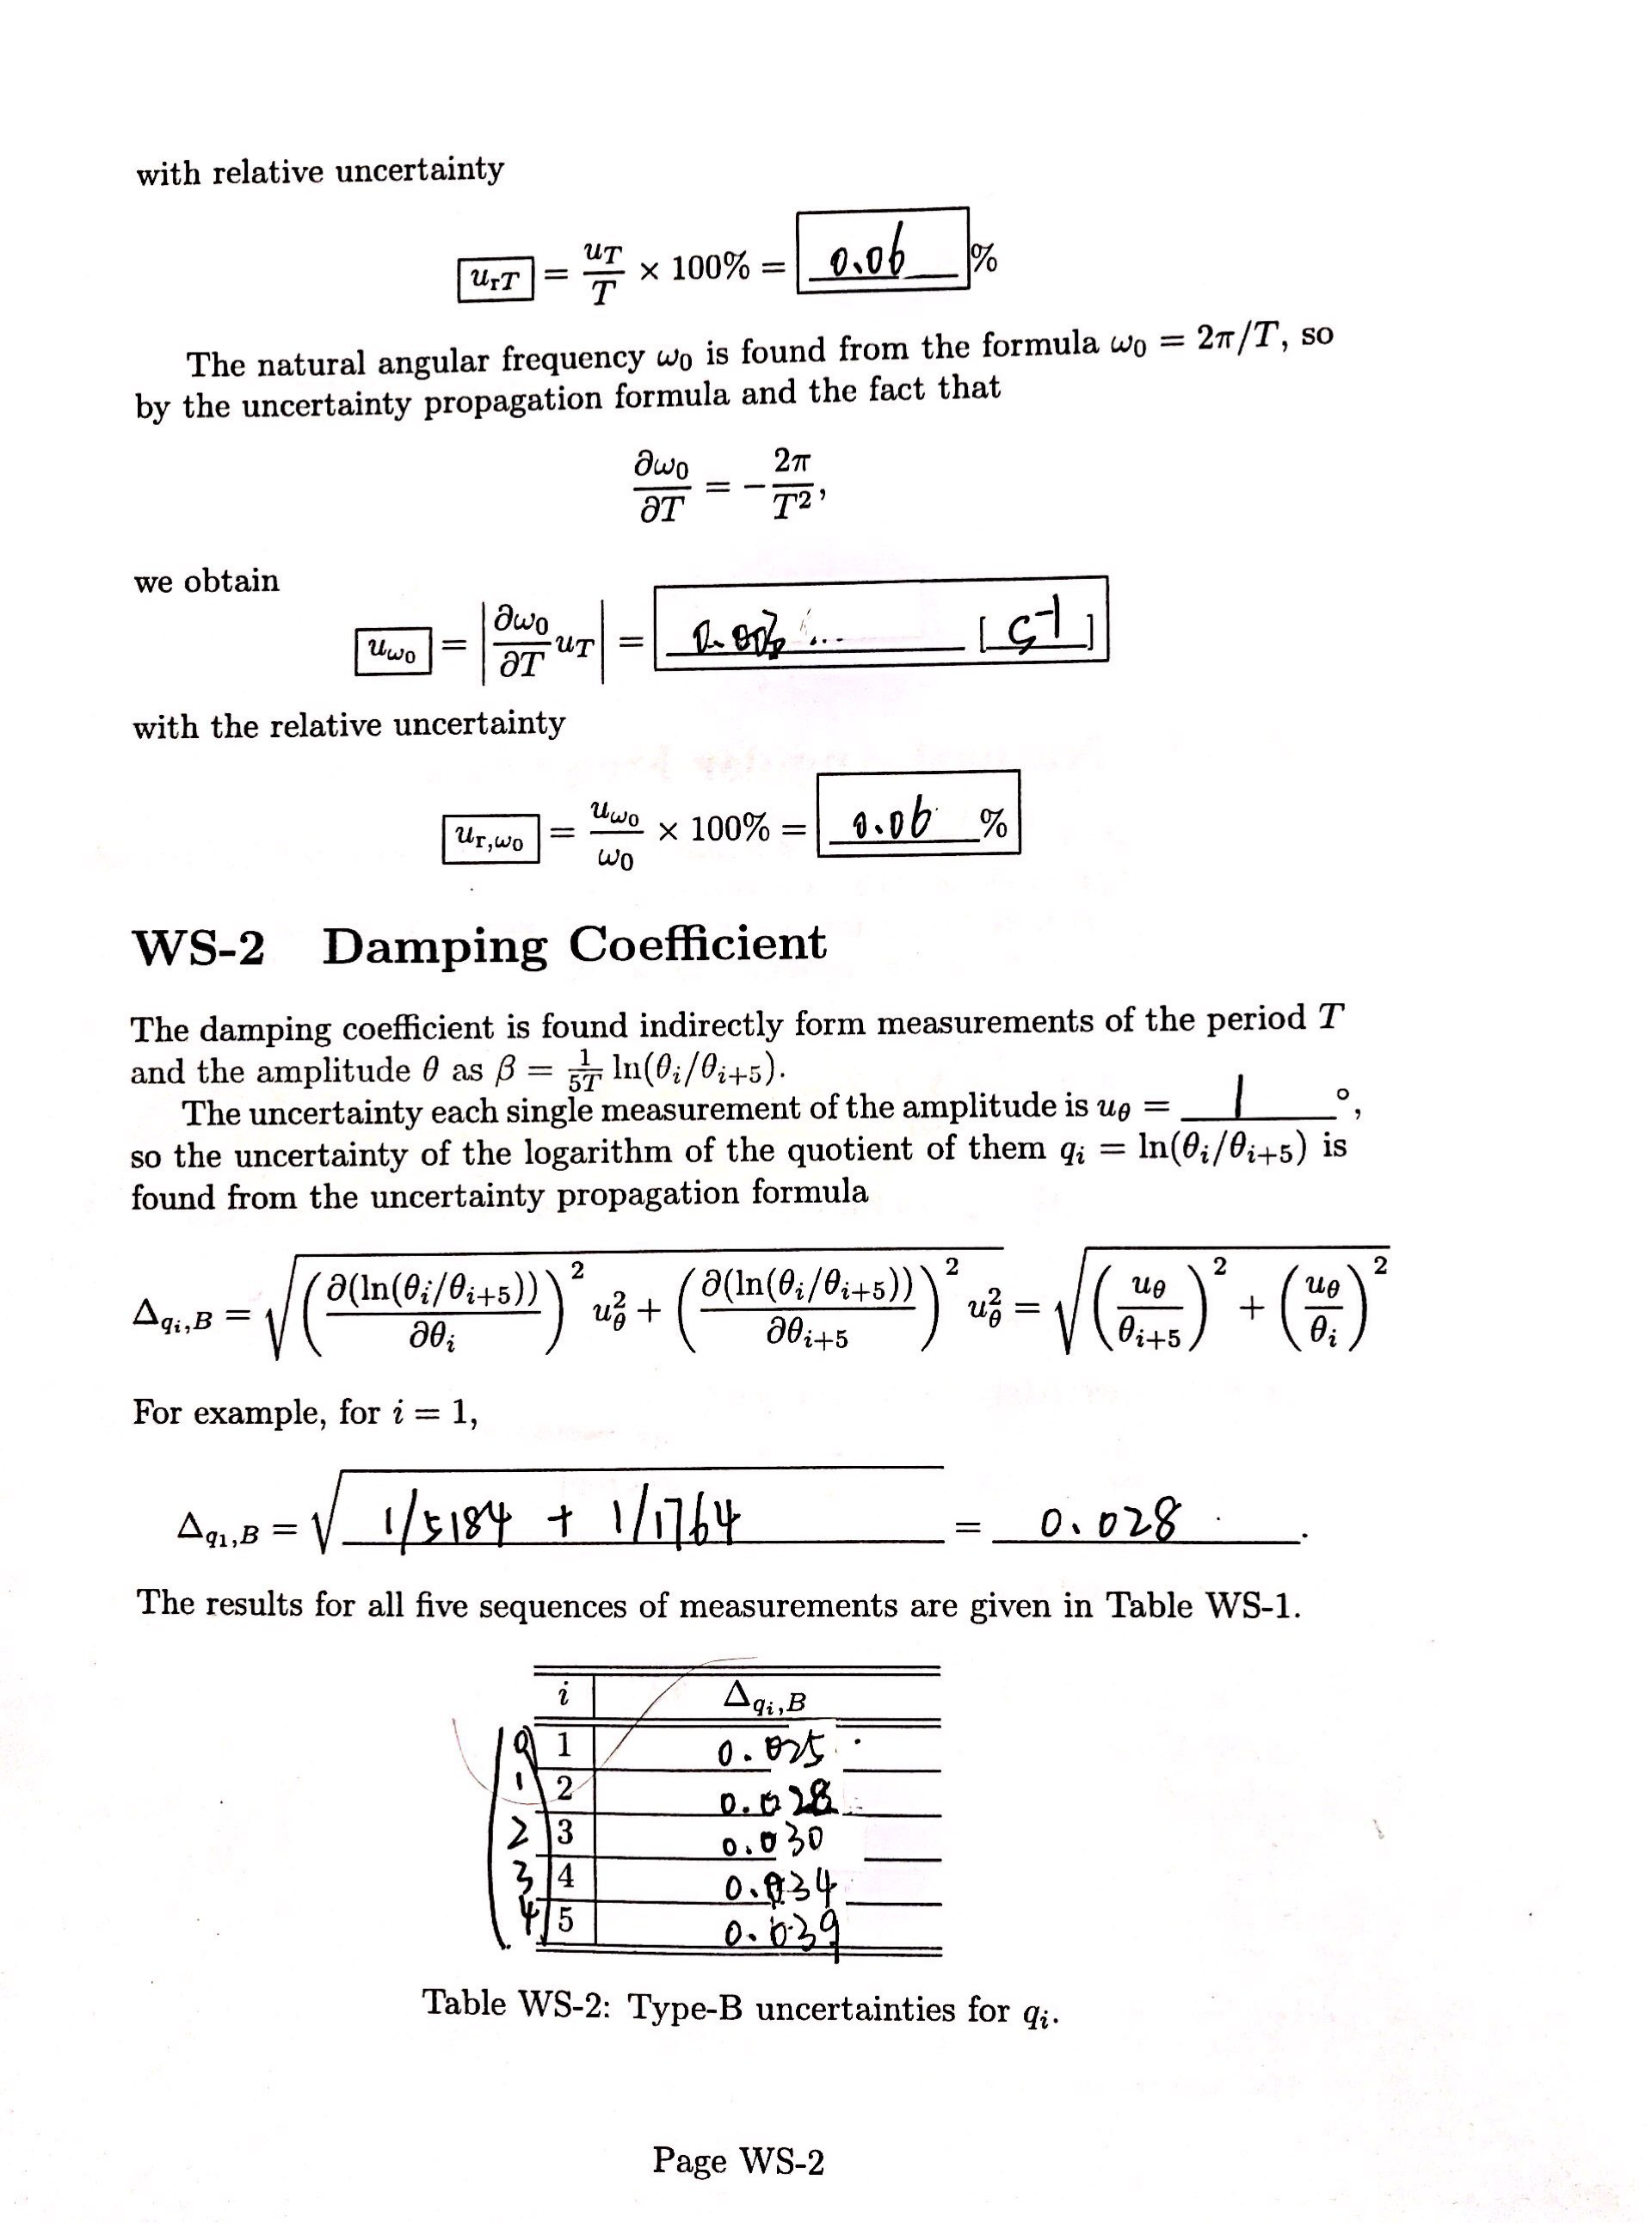
\includegraphics[scale=0.25]{newuncer2.jpeg}
\end{figure}
\begin{figure}[t]
    \centering
    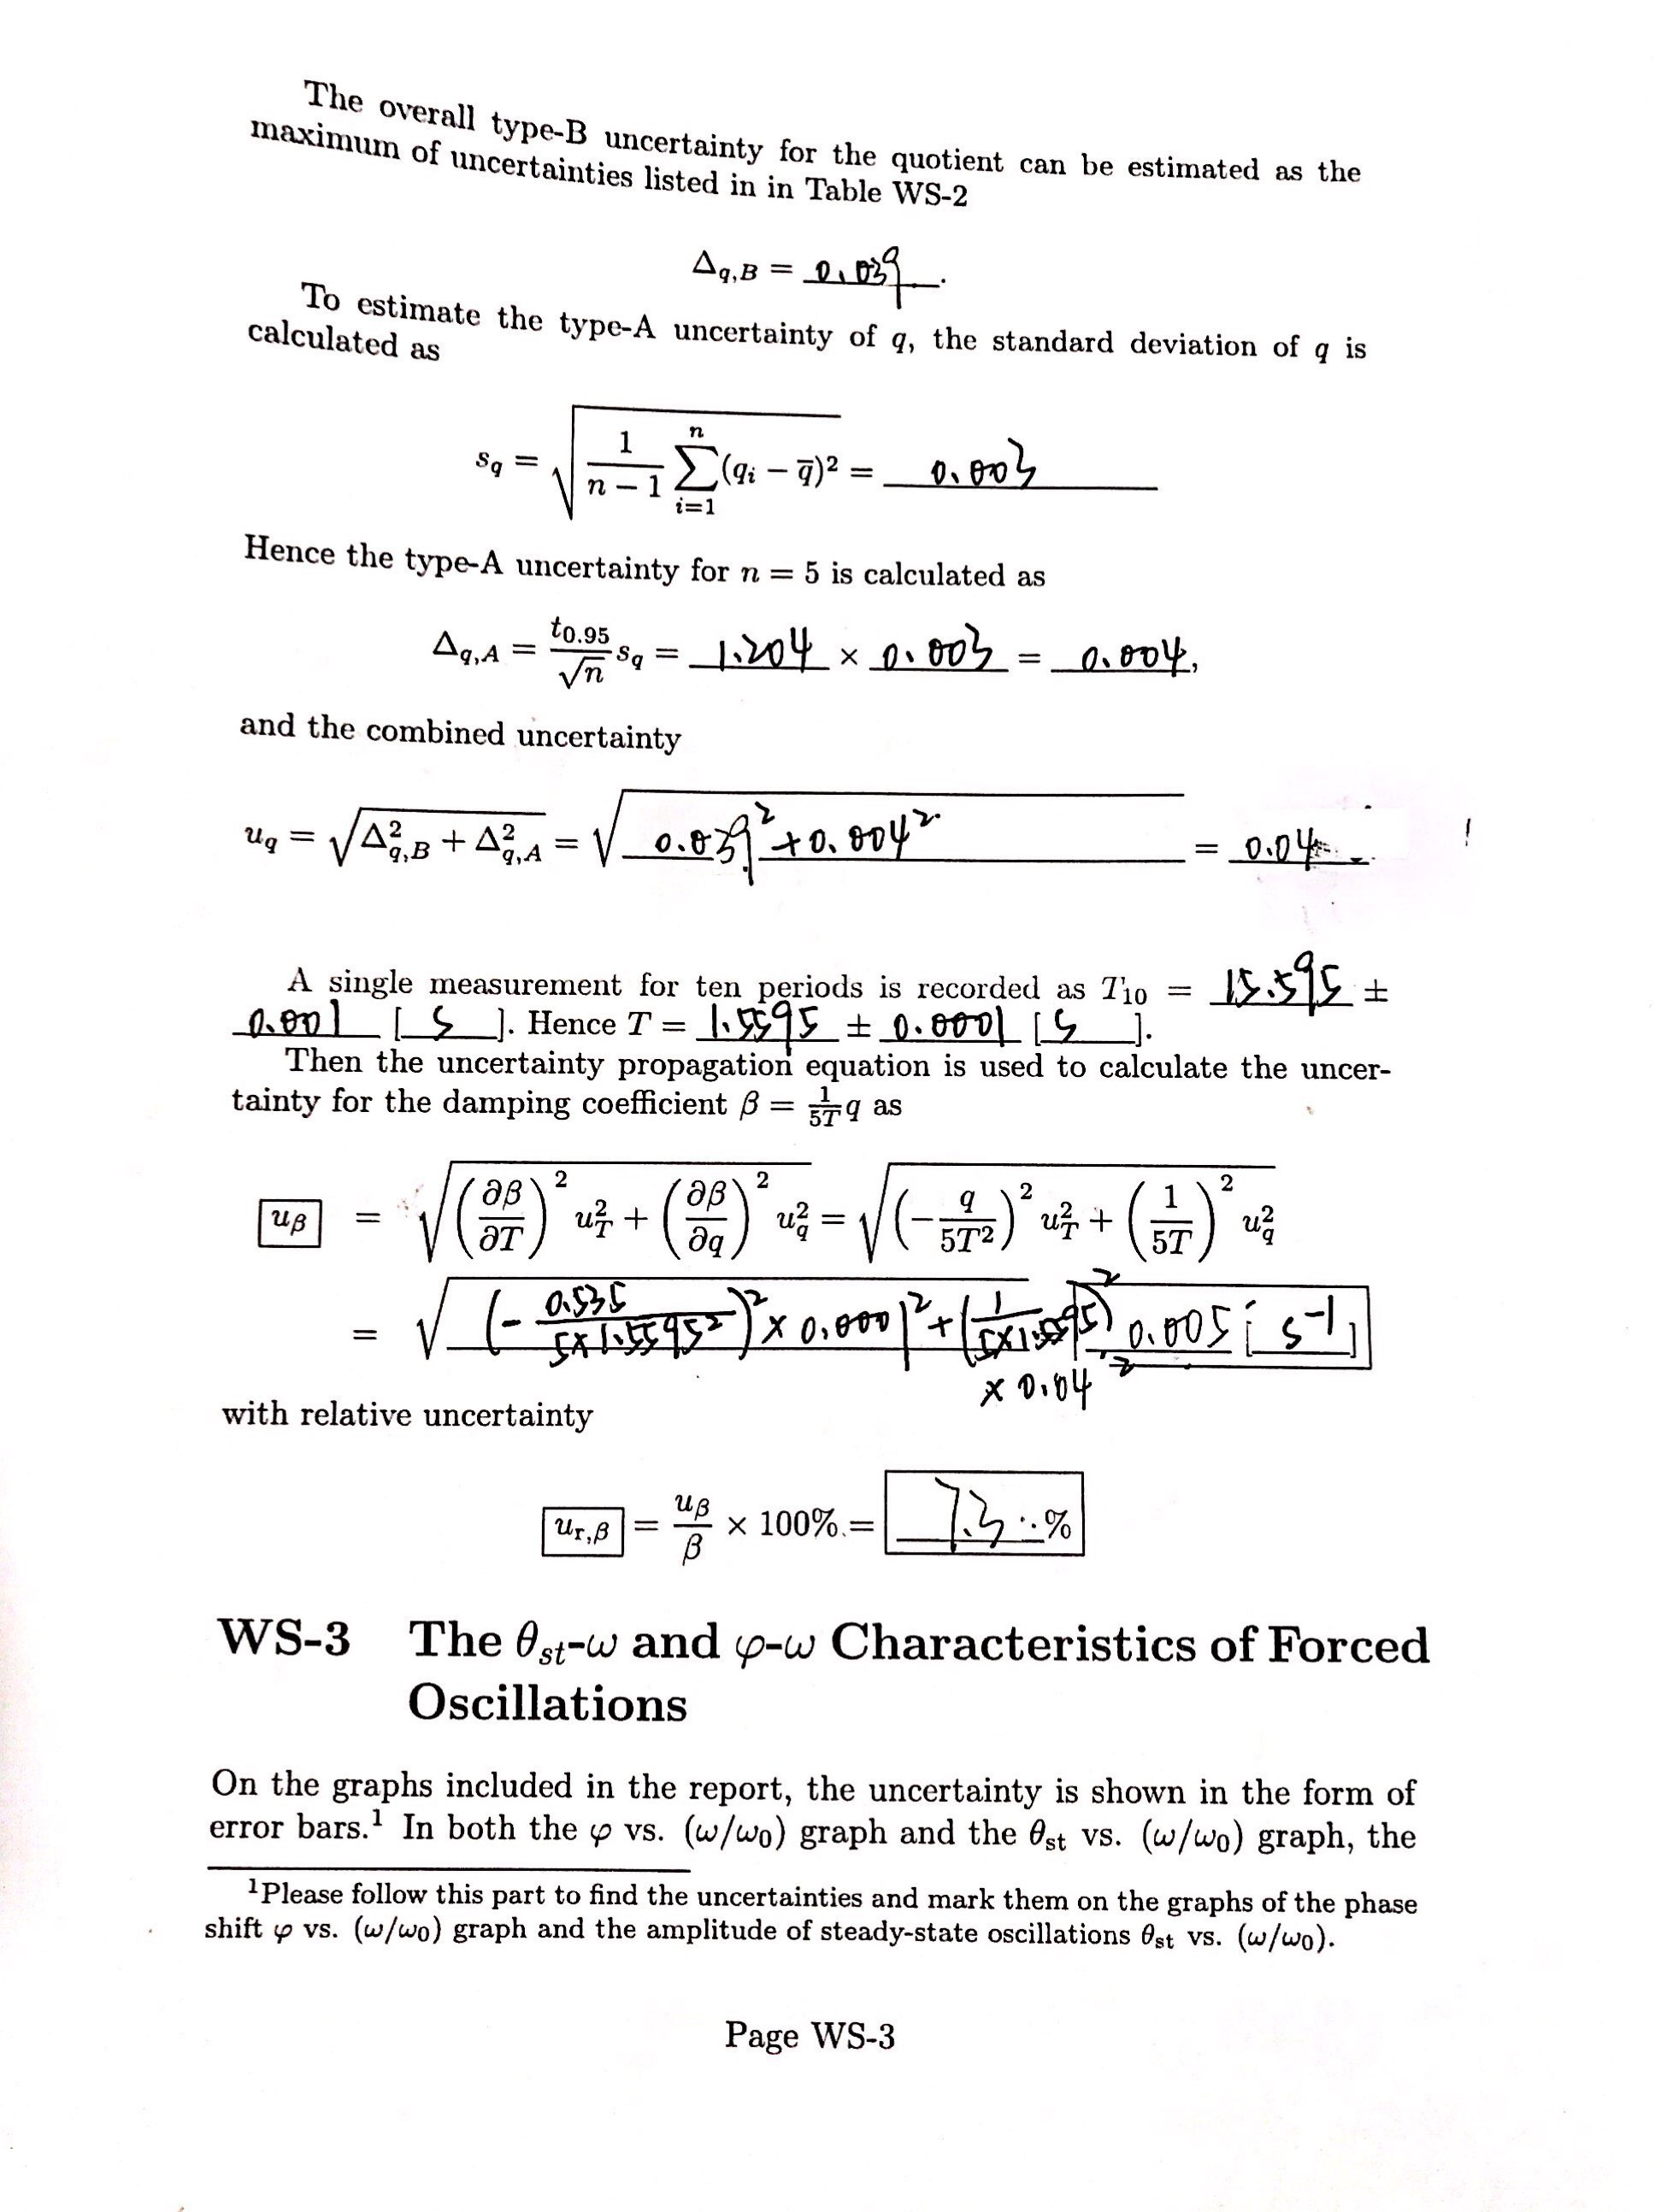
\includegraphics[scale=0.25]{newuncer3.jpeg}
\end{figure}
\begin{figure}[t]
    \centering
    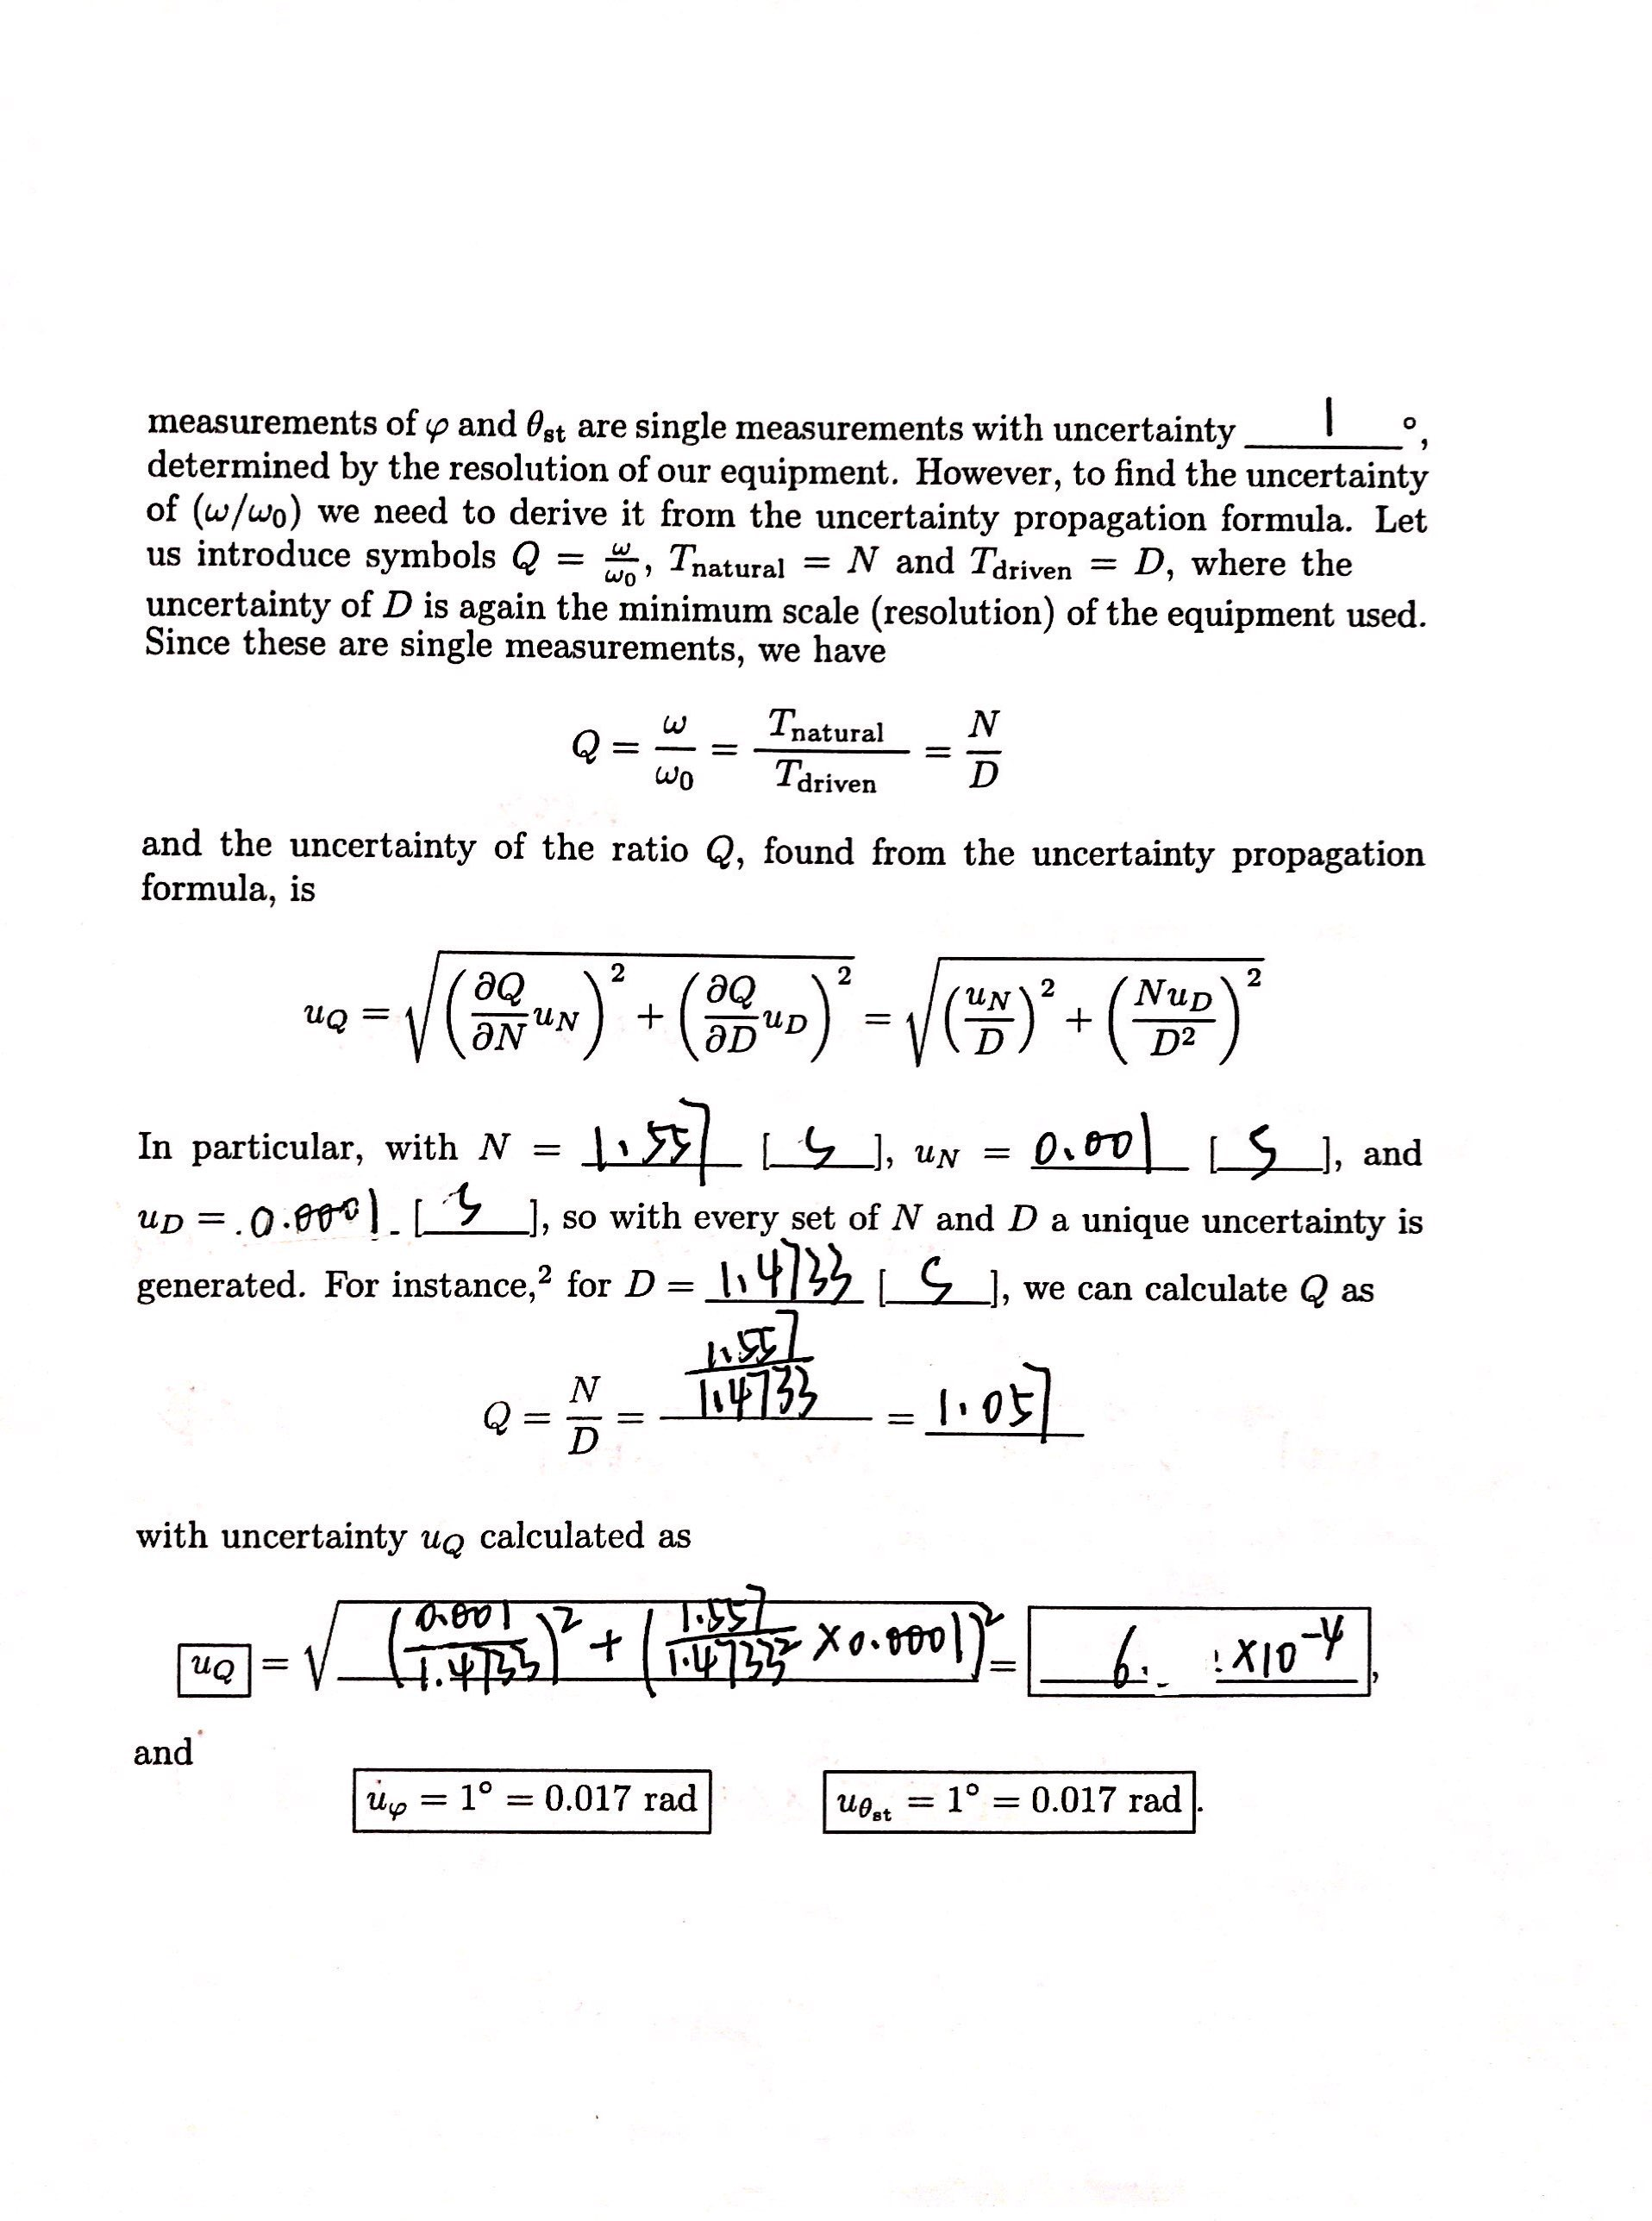
\includegraphics[scale=0.25]{uncertainty4.jpg}
\end{figure}
\end{document}